% 第五章 教皇使团和康熙派出的洋钦差
% 原书页码：155；标题
\section{教皇使团和康熙派出的洋钦差}
\par
% 原书页码：155；段落
1704年11月20日，教皇克莱孟十一世（ClementXI，1649—%
1721）签署了教内的禁约，禁止天主教徒参与中国传统的礼仪活动。明%
朝末年以来，不同天主教教会，甚至不同的传教士个人，在如何界定一%
些中国传统的仪礼上存在着分歧。比如，中国人在家里供奉死去亲人的%
牌位，在牌位前面上几支香，或者在家里供奉孔子的画像，这些算不算%
天主教教义里不允许的偶像崇拜？中国传统的习俗跟一神论的天主教%
有没有冲突？如果一个中国人皈依了天主教，婚丧嫁娶中哪些中国的%
传统仪礼他可以参与？哪些不能？这一大堆的争议，在天主教内部一%
直都没有定论。这些天主教内部的争论历史上称为中国礼仪之争。在%
中国传教的不同教会对许多问题都各有理解，互相说服不了，只好把%
各自意见发回到罗马教皇那里，让教皇仲裁。简单来说，认为可以允许%
信徒继续参与礼仪活动的一方认为中国的这些仪礼属于世俗层面，没%
有宗教层面的偶像崇拜意味，所以没有必要在教徒中禁止这些仪礼。%
\par
% 原书页码：156；段落
为了说服罗马教廷，耶稣会神父在1700年发了一个装着各种文%
件的大包裹去罗马。这里面包括他们翻译的儒家士大夫的论述，以%
及一篇他们写的并得到康熙认可的分析。作为旁证，他们还特意找%
到住在开封的犹太人，让他们写下了他们眼中的中国仪礼。不过教%
皇没有认同耶稣会神父的论点。为了尽快结束这个争论了半个世纪%
的话题，教皇签署了禁止教徒参与中国礼仪的谕令。不过，由于考%
虑到庞大的中国是很有前景的福音传播地，以及对于欧洲各国的国%
王来说中国在当时世界航海贸易中地位至关重要，教皇特地派了一%
个使团到中国来做沟通。%
\par
% 原书页码：156；段落
在1705年，首位教皇特使多罗到达北京之前，礼仪问题主要在欧%
洲争论。在华耶稣会士知道多罗到来以后，认为这是一个绝好的机会，%
可以在中国给多罗讲解中国礼仪，传达他们的观点。在华耶稣会士懂%
中文，也读了中国各种典籍，理所当然地认为在天主教世界，他们才%
是真正的中国通，他们才有资格解释中国礼仪，而教皇应该接受他们%
的观点。认为中国礼仪中有宗教意味的主要是天主教中多明我会的传%
教士（耶稣会内部也有神父反对中国礼仪）。他们的说法其实也有一%
定道理。比如拜祭孔子，拜祭中当然有尊师重道的意思，但是很多人%
祭孔时也在祈求孔子保佑能考取功名等。在天主教的教义中，他们是%
不能允许信徒对其他偶像祈祷的。还有拜祭祖先牌位这些，其中有没%
有祈求保佑的成分，都是很难说清楚的事。%
\par
% 原书页码：156–157；段落（跨页续段）
康熙也不是完全不知道欧洲在争论中国的礼仪问题。他或多或少%
从身边耶稣会神父那里听到一些风声。1700年，耶稣会神父在准备资%
料解释中国礼仪问题的时候，有一份论述就呈给了康熙过目，还让康%
熙签名支持了他们的观点。不过，康熙并没有把这些争论放在心上，%
也没有关注过。当听说多罗使团人华，他也没有想到过这个使团是来%
处理中国礼仪问题争论的。他最初以为多罗是来调解葡萄牙耶稣会神%
父和法国耶稣会神父之间的内部矛盾的，因为他知道双方有很多家长%
里短扯不清楚的问题。直到多罗人华半年以后，在康熙给多罗饯行那%
天，耶稣会神父才把问题报给康熙，希望康熙出面支持他们的观点，%
要求多罗把他们关于中国礼仪的意见带回到教皇那里。不过耶稣会神%
父把问题捅到康熙那里以后，整个事件走向就改变了。康熙作为大清%
皇帝立马把这个问题当成他自己的事，参与到了争论中去。%
% 原书页码：157；标题
\subsection{康熙和他的江山}
\par
% 原书页码：157；段落
1705年，康熙五十一岁。从铲除鳌拜算起，他已经亲政三十七年。%
作为第二位在京的满人皇帝，康熙先是平定了持续八年的三藩之乱。%
之后他直接掌控了繁华的南方诸省。在平定台湾一年后，也就是1684%
年，康熙第一次南巡。到1705年，他已经五次南下，其间登了泰山，%
拜了孔庙，还祭了大禹陵。康熙用这些象征性的行动在收服中华文人%
士子的心。同时在南巡中，康熙也见识了江南的富足，感受了传统中%
国的人文地理，对他治下的南方有了感性的认识。%
\par
% 原书页码：157–158；段落（跨页续段）
南方平定后，康熙把主要精力放到了北方。除了一直和俄罗斯谈%
判，在1689年签订《尼布楚条约》以外，康熙的主要对手是准噶尔%
汗国的噶尔丹汗（1644—1697）。噶尔丹早年在西藏学佛二十年，在%
学佛修行方面是有造诣的，他的上师是藏传佛教的大德。噶尔丹在他%
哥哥僧格汗被杀后，还俗去当可汗，开始了他的草原征战生涯。噶尔%
丹坐稳了可汗的位置后，趁喀尔喀蒙古内乱之时，侵吞了喀尔喀蒙古%
的土地，势力挑战着清朝在草原上的权威。康熙招降过噶尔丹，但遭%
到了拒绝。%
\par
% 原书页码：158；段落
对于康熙来说，噶尔丹是大清的心腹大患。一来噶尔丹不是只会%
挽弓射雕的普通蒙古部落首领，他是有文化并得到西藏活佛暗中支持%
的可汗。\NoteRef{5}{1}噶尔丹的存在，时刻提醒着康熙当年女真金朝被灭的历史。%
原本被金朝压制的成吉思汗，在统一了蒙古各部后，反过来把金朝给%
灭了。所以康熙不能坐视噶尔丹壮大。但征讨噶尔丹有很多实际困难。%
朝廷上下都反对远征，因为大家都知道，在草原上的噶尔丹骑兵来去%
无踪，可以随时西撤。而大清要远征的话，远距离后勤补给也是很现%
实的问题。不过康熙还是力排众议，决定征讨噶尔丹，而且还是御驾%
亲征。为了彻底消灭噶尔丹，康熙三次亲自出大漠远征，足见他对噶%
尔丹的重视。在1696年第二次远征中，大清同时派出三支大军北上，%
意在包围噶尔丹部队。康熙亲自指挥中路大军，与士兵同吃同住，北%
出一千多公里，穿越戈壁大漠，直接迎战噶尔丹主力。噶尔丹得知康%
熙亲征以后，迅速西撤，不过正好碰上大清左翼大军。噶尔丹仅率几%
十残部逃脱。第二年，噶尔丹在康熙第三次亲征中再次兵败。有传说%
他最后自杀。后世还留传有他生前用藏文写下的诀别诗。诗中的内容%
是希望他的上师能够拯救他，让他有机会转世到能听闻佛法的地方，%
来世有机会研习佛法。%
\par
% 原书页码：158–159；段落（跨页续段）
康熙亲征剿灭噶尔丹后，声名在大漠中远播，使他成为名副其%
实的蒙古各部可汗的可汗。耶稣会神父在康熙三次远征中，都跟随%
在侧。在大漠晴朗的夜空下，耶稣会神父和康熙一起仰望星空，探%
讨学问。他们留下了详细的随军日记，是后世了解康熙远征最详细%
的资料。\NoteRef{5}{2}%
\par
% 原书页码：159；段落
以传统中国的家庭标准来看，1705年的康熙也是很成功的。他%
有十五个儿子，其中九个已成年，都是能文能武、独当一面的角色。%
康熙1696年亲征噶尔丹之时，有六个儿子随他出征。这个时期的康%
熙家庭和睦，后来困扰他的皇子争位之事还未开始。应该说此时的%
康熙家和国强、天下归一、名震四海。就连欧洲的哲学家这时期都%
在读康熙的故事，莱布尼茨还提出了康熙是“开明专制”君主的典范。%
\par
% 原书页码：159；段落
康熙收服天下靠的不仅是战争，在文化上，他也获得了多方的%
认同。对于传统的中国士大夫来说，康熙发起了整理传统中国文化%
的大项目，修《明史》、撰《康熙字典》、编《古今图书集成》等，%
这些文化项目改变了许多晚明士人对满人的看法。而在蒙古人眼中，%
康熙也是他们文化的捍卫者，特别是康熙支持当时蒙古人信仰的藏%
传佛教。由于家庭缘故，康熙从小就在藏传佛教影响下长大。他的%
祖母孝庄就是藏传佛教信徒。孝庄派去照顾康熙的苏麻喇姑更是虔%
诚的信徒，一生持戒。康熙五上五台山参拜也是当时藏传佛教界的%
佳话。\NoteRef{5}{3}康熙还两次重印藏文的全部《大藏经》来支持藏传佛教。后%
来西藏方面直接认定康熙是文殊菩萨转世，康熙也欣然接受了这个%
名号。\NoteRef{5}{4}同时，对于当时的欧洲传教士来说，康熙热衷欧洲的各种学问，%
还把各种西学书籍翻译成了满文，介绍给满人贵族子弟。所以无论%
是传统中国士人、蒙古的喇嘛，还是欧洲传教士，都觉得康熙是热%
衷他们文化的皇帝。%
\par
% 原书页码：160；段落
在1705年，无论是作为一家之主，还是作为一个横跨东亚中亚%
多文化区域的帝国皇帝，康熙都是成功的。他征战草原，留下了各%
种神话。他巡游江南，与各地士人谈笑风生，留下一段段佳话。一%
方面，康熙是个有执行力的皇帝，敢于力排众议，坚持自已的决定；%
同时，康熙也是个懂得周旋、很现实的统治者。他与俄罗斯长达十%
年的谈判就是例证。康熙在知道藏传佛教支持噶尔丹后，他也派人%
去暗中处理。\NoteRef{5}{5}了解了康熙的基本背景，才能真正理解康熙在与教皇%
使团谈判中言行背后的含义。%
% 原书页码：160；标题
\subsection{康熙眼中的教皇使团}
\par
% 原书页码：160；段落
一直以来，多罗使团都被看作第一个代表罗马教廷来华的外交使%
团。但实际上，这是后人的误读。\NoteRef{5}{6}康熙从头到尾都没有把多罗使团当%
成外交使团，也没有通过任何朝廷部门来接待他们。康熙选用的是私%
人家庭会见的形式来和多罗使团见面，选用这种方式是基于他和传教%
士的关系。因为多罗是耶稣会传教士想要康熙接待的人，而耶稣会神%
父又是他内务府门下之人，所以作为一家之主的康熙接待多罗就像他%
其他奴才的亲戚来了，他用家庭方式接待是一样的。由于是家庭会见%
形式，接待多罗使团前后的全部安排都是内务府包办的，整个过程没%
有朝廷官僚系统的任何部门参与。\NoteRef{5}{7}%
\par
% 原书页码：160–161；段落（跨页续段）
耶稣会士第一次知会康熙多罗入华是在1705年6月。在接到耶%
稣会神父的汇报时，康熙出外打猎去了，不在北京。那时候多罗使团%
已经以商人名义交了该交的关税，进人了广州。也是这个原因，广东%
那边的官僚并没有注意这个使团，也没有向礼部通报。按照多罗的指%
示，耶稣会神父向康熙介绍多罗身份时，说他是圣教巡视官，是教皇%
派到各地检阅传教士所传教法是否合乎罗马教规的教皇钦差。康熙收%
到耶稣会神父的奏报后，并没有兴趣接见多罗，认为多罗是来检阅他%
们自已宗教的，跟他没有什么关系。康熙让他在北京的奴才把这个意%
思传达给了耶稣会神父。耶稣会神父跪下恳求，大意是康熙接见多罗%
实际是给他们所有在华传教士长“脸面”，希望康熙能够成全。说到%
“脸面”，康熙大概明白了，说是看在“豢养尔等多年”的分儿上，就%
接见一次。\NoteRef{5}{8}%
\par
% 原书页码：161–162；段落（跨页续段）
康熙收到传教士的奏报后，第一直觉是这个圣教巡视官是来调节%
北京耶稣会神父内部矛盾的。康熙知道耶稣会神父大概按国籍分成两%
派，一派是法国耶稣会士，一派是葡萄牙耶稣会士。康熙多次为他们%
处理过内部矛盾，总体认为就是些家长里短的小事。康熙和他身边的%
奴才说过，清官难断家务事，他根本不想管他们之间那些事。罗马现%
在还存有一道康熙的圣旨，里面专门说到他不能总是给耶稣会士断他%
们的家务事。\NoteRef{5}{9}康熙是懂人情世故的皇帝，在他看来，耶稣会神父之间%
的是非曲直不可能真的理清楚。要搞明白他们之间的问题，就要翻出%
很多陈年往事，这样很大可能会把各种矛盾激化，从而进一步破坏耶%
稣会神父之间的关系。康熙认为耶稣会神父之间的矛盾根本就不值得%
去调解，冷处理为上。同时康熙还知道，两边耶稣会神父各有教堂，%
入教的天主教徒，因为入的教堂不同，也互相有矛盾。用康熙的话%
说：“凡入南堂之国人，则骂入西堂之人；而入西堂之人，则骂入南堂%
之人。”\NoteRef{5}{10}想到这些问题，康熙认为要是圣教巡视官再把教徒之间的问%
题掺杂进去，麻烦就更大了。康熙写了封信给赫世亨。赫世亨是康熙%
身边的家奴，是内务府里负责与传教士打交道的奴才。康熙让他去找%
所有耶稣会神父确认，是否他们全体都同意接待多罗。\NoteRef{5}{11}同时他要找%
耶稣会神父问明白：为什么天主教人华都一百多年了，从来没听说过%
什么圣教巡视官，而现在突然教廷派了个这样职位的人来。康熙想知%
道是不是耶稣会神父在中国做了什么错事，传到罗马去，罗马派人来%
处理了。简单来说，就是康熙首先想搞明白这个人到底来中国是干什%
么的。同时康熙把巡视官来华断是非的猜想说出来，让赫世亨转告传%
教士。这样对传教士也是一个警告，意思是如果你们各方都同意接待，%
那你们就要互相容忍，达成共识。\NoteRef{5}{12}%
\par
% 原书页码：162；段落
1705年7月23日，赫世亨把北京耶稣会神父召集到一起，问了%
他们康熙要问的问题。耶稣会神父在跪拜感恩康熙的询问以后，首先%
解释这个圣教巡视官来华的主要目的是感谢康熙容留传教士和天主教%
的。第二，他们确认所有神父都赞同接见多罗。第三，他们保证已经%
互相协调好了彼此的关系。最后，他们解释多罗是个虔诚的修教之人，%
很年轻时就已经开始当神父了。\NoteRef{5}{13}%
\par
% 原书页码：162；段落
康熙接到赫世亨的汇报以后，在回复中提到，这些北京耶稣会神%
父说的跟他身边耶稣会神父龙安国等人说的有出人。具体有什么出人，%
康熙没有明示。康熙批注说，看在多罗确实是神父身份，就让他进京。%
同时康熙吩咐赫世亨进一步询问北京耶稣会神父，希望自己如何接待%
多罗，以及多罗一行人现在是何种穿戴。\NoteRef{5}{14}%
\par
% 原书页码：162–163；段落（跨页续段）
北京耶稣会神父很惊讶康熙还要询问他们的意见，除了表示受宠%
若惊以外，他们说如何接待都听皇上安排，皇上能够接待就已经是天%
恩了。同时他们也不知为何康熙要询问多罗一行的穿戴，只就他们知%
道的圣教巡视官去罗马以外的欧洲国家是何种穿戴做了一个笼统的回%
答。赫世亨在汇报了北京耶稣会神父的回答后，最后加了一句，大意%
说，据他观察耶稣会神父回答问题时的神色表情，他们确实在如何接%
待上没什么要求（“观伊等之神态，确实以诚心恳请于皇上”）。\NoteRef{5}{15}%
\par
% 原书页码：163；段落
其实康熙问这两个问题是有深意的。站在康熙角度，接待这个使%
团有两个方式：一是用传统接待外国使团的方式，通过朝廷安排，走%
既定流程；二是私下由他的内务府当作他的家庭聚会来安排。既然传%
教士之前提到，希望康熙接待的目的主要是给他们长脸，康熙自然想%
到他们是否希望要通过朝廷，在紫禁城的大殿中来接待。康熙问多罗%
一行人是如何穿戴，其实是想知道这些人到底穿的是宗教服装，还是%
外国使节的服装。%
\par
% 原书页码：163；段落
知道耶稣会士对接待方式没有特别要求后，康熙认为事情就简单%
了，直接批注多罗一行不是外交使节，不算西洋来的外国使团。而且%
命令他们北上时穿中国样式的衣服，这样就减少了一行人是外国人的%
直接观感。康熙的原话是多罗一行“并非西洋王等所差进贡之人，因%
而着穿我此地衣服”。\NoteRef{5}{16}这样康熙就给这个使团定了性，它不是外交使%
团。康熙让赫世亨在去办理接待前，最后和耶稣会神父确认了一下，%
整个安排他们是否满意，是否还有什么遗漏。耶稣会神父接到赫世亨%
的传话后，当然又是千恩万谢感恩戴德，只是最后提了一个小请求，%
就是在安排使团北上的行程时，尽量能给安排水路，因为欧洲人并不%
像满人那样能够长时间骑马。\NoteRef{5}{17}%
% 原书页码：164；标题
\subsection{初次接见}
\par
% 原书页码：164；段落
由于是康熙私下家庭内部接待，朝廷各部门对接待教皇使团的全%
部过程没有任何记载。现有几封康熙包衣奴才给康熙的满文奏报，让%
我们可以大概了解康熙是如何全面绕开朝廷部门的。权力运作，任何%
安排都离不开通讯联系。康熙要安排一个外国使团从广州到北京，命%
令可以畅通传达是运作的核心。朝廷的官僚系统中，北京与地方有专%
门的通信驿站，可以互相联系，这是自古就有的。这之外，康熙和他%
在一些地方做官的包衣奴才还有私下的通信渠道。一般是由地方上包%
衣奴才直接派他们的家人把信送到北京，由内务府的人或是特定宫中%
侍卫来接收这些信件。这样一来，这些信不经过朝廷任何部门，就直%
接送到皇帝手里了。后来雍正朝的密折制度就是在这种通信联络方式%
下发展出来的。这种联系具有私密性，皇帝主要用此来处理比较隐秘%
的事，或是需要保密的军务。%
\par
% 原书页码：164–165；段落（跨页续段）
接待教皇使团，属于公开接待，不需要保密，而且地方上的接待%
过程需要彰显大清皇帝的面子，这就决定了皇帝和地方官的私密联系%
不适用这种情况。同时全部安排又要绕开朝廷，这样走朝廷的通信网%
络也是不恰当的。康熙在接待教皇使臣上，展示了第三种北京和地方%
的联系方法：宫里派人去找到各地方官在北京的亲戚，让这些亲戚通%
过自己家族内部的联系渠道，去通知地方官员。在外面避暑的康熙，%
发信给留在北京的赫世亨，让他把事情“饬交总督巡抚子弟”去办理。%
赫世亨后来在给康熙的信中汇报说，他在北京找到了“总督族侄郭朝%
宾，巡抚之子内阁中书石成峨”。报告中没说是哪里的总督和巡抚。%
不过，这二人的姓氏正好对上当时的两广总督郭世隆和广东巡抚石文%
晟。也就是说赫世亨是通过两位广东大员在北京的亲戚来联系二人的。%
赫世亨还告诉康熙，石成峨说他马上就去办理，但说现在沿途道路泥%
泞（当时是7月底8月初，正是夏天），需要多些时日。\NoteRef{5}{18}%
\par
% 原书页码：165；段落
可以想象两位广东大员接到他们在北京的子侄发来的康熙旨意%
后，肯定明白康熙守着现成朝廷的通信馆驿不用，而选择私下联系他%
们，其中所包含的深意。站在两位封疆大臣的视角，他们知道康熙这%
样联系他们，意味着他们需要在完成康熙的部署之外，还得把这件事%
情和为朝廷办的“公事”区分开来。这件事只能当成他们自己的私事%
来办，就像是他们家人请他们办的事一样。后来赫世亨在另外一份奏%
报中告诉康熙，根据北京传教士收到广州传教士的信中所说，广东巡%
抚已经收到北京发去的指示了，而且还带着当地官员去了教皇使节住%
的教堂。同时，赫世亨还在奏报最后附了一句，总督、巡抚都没有发%
文过来。这样相当于向康熙确认，总督、巡抚把事已经办妥了，而且%
他们也明白这件事的“私”事性质，没有发文到北京来。康熙看完以%
后，批注“知道了”。\NoteRef{5}{19}根据传教士的记录，广东官员收到皇帝通过他%
们亲戚发过去的指示后，款待了教皇特使。而且广东巡抚还自己出钱，%
给整个使团购买了中式衣服，让他们进京路上穿。\NoteRef{5}{20}这也从侧面看出，%
广东官员完全知道康熙的安排，也领会了其中的意思。%
\par
% 原书页码：165–166；段落（跨页续段）
内务府不止通知了两广官员，教皇特使多罗一行沿着运河北上，%
沿路的官员都有接应。多罗一行人从广州出发，经过三个月的跋涉，%
于1705年12月4日到达北京。根据当时去迎接多罗的耶稣会神父记%
载，一行人的行李繁多，装了13辆马车，外加80个挑夫。这么大的%
队伍，到哪里都是惹人注目的。多罗到北京后详细和耶稣会神父讲了%
他在沿途遇到的各地官员和王公贵族款待他的情况。有北京方面打招%
呼，多罗自然是一路顺风，外加各种礼遇款待。不过似乎多罗自己还%
以为是这些官员本性好客、和善，殊不知这都是皇帝的面子。%
\par
% 原书页码：166；段落
多罗进京后，一直生病。直到12月31日，康熙才安排接见了多罗。%
在接见当天，多罗一行在内务府安排下从故宫的西门进人。接见安排%
在下午两点，地点是在故宫北面景山下的某处园子。\NoteRef{5}{21}%
\par
% 原书页码：166；段落
整个故宫是按古代风水理论坐北朝南设计修建的，皇帝各大殿中%
坐的龙椅都是面向南方。大臣、外交使节，按朝廷礼仪，是从故宫南%
面过午门再进太和门来拜见皇上。同时，正式的朝廷接见一般安排在%
故宫正中富丽堂皇的太和殿，时间安排在上午。而多罗一行，走的是%
内务府专用的西门，会见地方也是在皇帝平时游玩的一处园子。整个%
时间地点和路线安排，都符合康熙最初策划整件事情的定位：这是一%
次私人的聚会。%
\par
% 原书页码：166–167；段落（跨页续段）
尽管是康熙安排的私人会见，全程还是礼数周到，尽显大清的皇%
家气场。康熙派出侍卫护送多罗一行人宫，路上还有很多围观外国人%
的老百姓，侍卫还需要不停驱散人群，为多罗一行开道。多罗是坐着%
轿子，被抬到距离会见不远的地方。轿子放下来以后，康熙的太监迎%
上来，跟多罗最后确认接见中的礼数等细节。康熙跟耶稣会士相处几%
十年，知道欧洲人到中国后，对中国三跪九叩的礼节有顾虑。早在%
三十年前的1676年，俄罗斯使臣人京，就和礼部官员为这叩头的礼%
节来来回回争论了很久。康熙自已对这一点是很通融的。现在整个接%
见又没有经过朝廷部门，他便让太监直接告诉多罗，他可以自已选择%
用中国的跪拜方式，或者欧洲屈膝的方式来行礼。\NoteRef{5}{22}%
\par
% 原书页码：167；段落
多罗选择了欧洲的方式，屈膝躬身给康熙行礼。康熙盘着腿坐在%
垫子上用满人的方式接见了多罗。很快，康熙和他身边的太监都发现，%
多罗身体还未恢复，很难像康熙一样盘腿坐在地上的垫子上。但太监%
又发现当时的场景下，给多罗抬一把中式的椅子也不妥当。因为坐在%
椅子上，多罗就比康熙高出一截。最后太监想到一个办法，把几个垫%
子叠在一起，给多罗拼出一把小凳子。这样整个会见还是在预先设定%
的满人家庭接待的方式下进行的。\NoteRef{5}{23}%
\par
% 原书页码：167；段落
作为家庭接待，现场没有任何朝廷官员。康熙当时还向多罗专门%
强调了这一点，告诉多罗在座都是他自己人（耶稣会神父），让他放松，%
不要拘谨。康熙还告诉多罗把这次聚会当成家庭聚会，该说就说，该%
笑就笑，不要有顾虑。双方说了一些客套话以后，康熙让太监端出了%
奶茶（在场神父的记录是有牛奶的茶），以及各种点心共计三十五道。%
在场的翻译法国传教士张诚告诉多罗，康熙只有接见他的家人亲戚时%
才会如此安排。\NoteRef{5}{24}%
\par
% 原书页码：167–168；段落（跨页续段）
整个会见气氛融洽，多罗也很得体地多次感谢康熙对天主教的包%
容，以及对传教士的各种照顾。吃喝了一会儿，康熙觉得多罗比较放%
松以后，询问多罗有没有特别的事要向他面陈的。自从知道多罗人华%
以后，康熙就一直在琢磨这人到底是来中国干什么的。在会见前几天，%
康熙专门派人去问了多罗有没有什么文件要送呈的。当时多罗写道：%
他是专门人华来感谢康熙对天主教的包容的。康熙看完后，对身边的%
人说，这肯定不是真实目的。\NoteRef{5}{25}康熙认为教皇不可能派这么庞大的一%
支队伍跋涉万里，跑到中国来谢恩。康熙认为他们肯定有什么特别的%
任务。同时，康熙又认为多罗写出来可能有顾虑，只愿意面陈。所以%
他在会见中，又问了这个问题。听到康熙的提问，多罗又是一通客套%
话后，说他人华还有个目标，就是希望建立一个特别联络处，来加强%
教皇和康熙之间的联系。同时多罗还补充说，这个联络处还可以便利%
大清和欧洲各国之间的贸易。\NoteRef{5}{26}欧洲知道俄罗斯在北京设立了一个办%
事处，一直很羡慕，所以多罗认为自已要是能在北京谈下一个这样的%
联络处，可以大大提升教廷在欧洲的地位。康熙对建立联络处的想法%
并不反对，只是说联络处建立只能是应对宗教相关的问题，不能涉及%
贸易方面。\NoteRef{5}{27}2%
\par
% 原书页码：168；段落
这时候，双方对联络处人选有不同意见。在康熙看来，要成立这%
样的联络处，人选肯定要从他周围的耶稣会传教士中选取。但康熙发%
现多罗似乎不想在耶稣会神父中选人，要另找。这时康熙以为多罗对%
耶稣会神父有不满，于是便开始夸奖耶稣会神父，为他们说了一大堆%
好话。不过康熙从谈话中察觉多罗还是不愿意用耶稣会神父后，就把%
话题岔开了。最后，康熙专门和多罗强调，他认为耶稣会神父从明代%
人华以后，所言所行，都无可挑剔。康熙让多罗把他这个评语带回去，%
转达给教皇。最后，多罗恳请康熙能一如既往地优容传教士。康熙回%
答说，只要他们遵守大清的规矩，他自会善待他们。\NoteRef{5}{28}28%
\par
% 原书页码：168–169；段落（跨页续段）
会见结束后，康熙立马私下把安多、徐日升、张诚三位神父叫到%
他那里。这三人都是跟了康熙多年的传教士。徐日升1673年人京，%
已在康熙身边32年；安多20年；张诚16年。康熙见到三人，便开门%
见山地说他认为多罗不信任他们。而且康熙想知道他们与多罗之间到%
底有什么问题。站在康熙的角度，他确实很不解。多罗是这些耶稣会%
神父引荐给他的，而多罗竟然又不相信他们，貌似对他们有不满。耶%
稣会神父知道多罗对他们有意见。多罗到京以后，已经和耶稣会神父%
会见过好几次，多罗对他们在中国的很多行为都有意见，几次会见都%
在争吵中不欢而散。不过面对康熙，传教士还是不想张扬他们自已内%
部的问题。安多在康熙面前说，多罗表扬过他们，说耶稣会是天主教%
内部最虔诚遵守戒律的教会。康熙听后半信半疑，向另外两位神父求%
证。另外两位点头称是。康熙似乎还是不相信，但也理解神父也许是%
不愿家丑外扬，便没有继续深问。康熙补充说，只要你们北京神父觉%
得没问题就行，反正接见多罗也是看在各位北京神父的面子上。\NoteRef{5}{29}%
\par
% 原书页码：169–170；段落（跨页续段）
16世纪初，欧洲基督教内部出现了分裂，一部分基督教徒不认可%
教皇权威，成立了新教。新教迅速在欧洲发展，后来荷兰、英国都变%
成了新教国家。耶稣会1540年成立的背景就是为了宣扬天主教、对%
抗新教在欧洲的扩展。耶稣会成立之时，正值全球航海时代兴起，因%
而该会还有一个宗旨就是把天主教传播到世界各地。耶稣会成立时有%
七位元老。七位元老之一的沙勿略神父就亲自远赴亚洲传教，先后去%
过印度和日本，最后在准备进入中国时去世。他去世时在上川岛，该%
岛现属广东台山市。耶稣会到世界各地传教，就要融入各地社会文化，%
在这个融入过程中，他们有些做法被天主教内部其他协会认为是不符%
合天主教教义的。特别是1622年教皇格列高利十五世（Gregory XV，%
1554年1月9日—1623年7月8日）成立了传信部（Sacra Congrega-%
tio de Propaganda Fide）来规范和监督去往世界各地的传教士的所言所%
行。当时在世界各地传教的耶稣会，也就成了传信部重点监督的对象。%
多罗就是传信部派出来的神父。\NoteRef{5}{30}多罗自己在罗马教廷内部地位很高，%
同时又是教皇钦定派出的巡视官，他自然认为北京耶稣会神父都应该%
听他的教诲和安排。到北京后，多罗指出了耶稣会神父的许多问题。%
比如耶稣会神父在中国买田置地，然后用来收租，这一点有违教义。%
特别是耶稣会神父和当地人签订的租赁合同，在多罗一字一句的审视%
下，有很多违背教义的地方，这些都需要整改。尽管耶稣会神父表面%
上态度恭敬服从，但心里是不服的。他们只承认多罗的职位比他们高，%
但不认为在天主教教义的解读上多罗比他们更有发言权。多罗到了北%
京，跟北京传教士发生多次争论，很多整改意见他都没办法落实下去，%
这也是他不信任耶稣会神父的一个原因。%
% 原书页码：170；标题
\subsection{教皇使节与传教士}
\par
% 原书页码：170；段落
多罗在与康熙的第一次会见中，表示出对耶稣会神父的不信任，%
实际是因为他当时还不知道耶稣会神父在京城中的能量，也不知道%
他们在北京和康熙皇帝之间的关系。北京传教士能够接触到康熙皇%
帝，多罗是知道的。但在多罗的认知中，能接触到皇帝的传教士并%
不稀奇，在欧洲，能接触到国王的传教士有很多。但让多罗想不到%
的是，这些传教士在康熙的眼中，是他内务府中之人，也就说是他%
的自己人。%
\par
% 原书页码：170–171；段落（跨页续段）
耶稣会神父和康熙的府内关系，多罗是在和康熙的交流中一步步%
明白的。康熙在接见多罗中，尽管对多罗不信任耶稣会神父有点奇%
怪，但总体上他认为多罗是得体的，同时也愿意借着这个机会，进%
一步和教皇发展关系。康熙提议他也派出一个使团，给教皇回送礼%
物。最初康熙决定派一个他身边的内务府包衣奴才带着礼物去欧洲。%
但是这个包衣奴才和康熙讲，他一种欧洲语言都不会，不能和任何%
人交流，他去欧洲没有办法传达康熙的意思。\NoteRef{5}{31}康熙觉得语言确实是%
个问题，于是决定派耶稣会神父白晋做他的特使去欧洲。白晋已经%
做过一次康熙的特使，在1690年代返回过欧洲去招募更多传教士到%
中国。所以康熙决定这一次再派白晋当他的特使。多罗听说康熙要%
派使节去拜见教皇很高兴，他把这看作是他出使中国的功劳。但当%
得知康熙指派了一位耶稣会神父去罗马，他不放心，于是在他的使%
团中选出了沙国安神父，让他和白晋一起同去欧洲。由于多罗总体%
上不信任耶稣会神父，他就让沙国安神父作为负责人来运送康熙的%
礼物。同时，多罗还写了一封长信，汇报他与康熙会面的情况，准%
备让二人把信带给教皇。信写好后，翻译了出来，多罗交给康熙过%
目。康熙看完以后，让赫世亨带话给多罗，告诉他，信总体内容很好，%
唯独信中最后把白晋说成沙国安神父的助手，这一点不妥。\NoteRef{5}{32}赫世亨%
向多罗转达康熙的意思：%
\par
% 原书页码：171；段落
{\bookkai 为了显示对教皇的敬意，我特地选派了我御前之人白晋。白晋是}%
{\bookkai 真正侍奉我左右的人，所以我选他代表我把礼物送给教皇。当然，白}%
{\bookkai 晋跟你们其他人一样，是个神父。但不同之处在于他是在我身边服侍}%
{\bookkai 多年的人，也是我府内之人。我让他全权代表我赠送礼物给教皇。\NoteRef{5}{33}}%
\par
% 原书页码：171–172；段落（跨页续段）
派身边的亲信和亲近奴才出使，是满蒙的老传统，这和汉人传统中派%
有身份的官员出使不同。这也是为什么康熙强调白晋是他“御前”之%
人这一点，而白晋在朝廷中没有任何官职。%
\par
% 原书页码：172；段落
多罗似乎不完全明白派亲信出使的意味，也不明白康熙强调这个%
“御前”之人的意义，因而他只是把信中的措辞稍微修改了一下，实%
际上还是让沙国安负责带领整支队伍，并把装有礼品箱子的钥匙也交%
给了沙国安。但在1706年6月，当白晋和沙国安两位神父到达广州，%
在那里等船去欧洲的时候，二人产生了矛盾，开始争论到底谁才是这%
个使团的主导，并把问题传回了北京，要北京给出明确指示。当时管%
理内务府的是康熙的大皇子，听到这个事情，当着众多传教士的面就%
发火了，说：%
\par
% 原书页码：172；段落
{\bookkai 这怎么可能是个问题？怎么可能有人对白晋是我们的使节有疑}%
{\bookkai 问？他在我们宫中二十年，满文中文都会，一直在父皇那里效力。而}%
{\bookkai 谁是沙国安？谁认识他是谁？\NoteRef{5}{34}}%
\par
% 原书页码：172；段落
当然康熙也是这个意思，肯定了白晋才是他的人。多罗在多方了解以%
后，也终于明白了康熙所谓白晋是他“府内之人”这个名号的分量。他%
也赶紧写信给沙国安，让他不要再和白晋争了，他信中和沙国安讲：%
\par
% 原书页码：172；段落
{\bookkai 我不得不提醒你，那位神父是皇帝真正的仆人，因而无论怎么让}%
{\bookkai 着他都是对的。\NoteRef{5}{35}}%
\par
% 原书页码：172–173；段落（跨页续段）
在欧洲的思维中，所有人都可以被称为皇帝的奴仆，所以皇帝的仆人%
可以是个礼仪性的称谓。现在多罗终于明白了，白晋是真正在皇帝身%
边干事的那种仆人，因而多罗称其为“真正的仆人”。%
\par
% 原书页码：173；段落
把事情闹大了，康熙还是下旨要求白晋克制，注意言行。白晋的%
满文检讨书发回了北京。这封检讨还在清宫档案里，以前将检讨书从%
满语译为汉语的翻译可能不知道白晋和沙国安互相争权一节，所以把%
白晋翻译成了博津。白晋的检讨如下：%
\par
% 原书页码：173；段落
{\bookkai 博津谨奏：}%
\par
% 原书页码：173；段落
{\bookkai 康熙四十五年五月十六日，赫世亨、张常住、赵昌传宣谕旨，六}%
{\bookkai 月十九日，博津我跪受。恭读明主训旨，始知我之所行最为无理。前}%
{\bookkai 日与沙国安同行，未有谦让，与之争先。我二人虽非不睦，但我无理，}%
{\bookkai 有违大主圣意，铸成大错。今我竭力仰副大主训谕，嗣后不敢与沙国}%
{\bookkai 安争先，必谦逊和气，断不违明旨，惟叩请仁主宽恕我此大罪。为此}%
{\bookkai 谨奏。}%
\par
% 原书页码：173；段落
{\bookkai 朱批：知道了。\NoteRef{5}{36}}%
% 原书页码：173；标题
\subsection{多罗与礼仪之争}
\par
% 原书页码：173–174；段落（跨页续段）
多罗到北京以后，其实还有一项任务，就是到中国来宣布和执行%
教皇关于中国礼仪的禁令，即不再允许入教的信徒继续参与很多中国%
传统的风俗活动。作为教皇特使，多罗本以为他有权对北京的耶稣会%
神父发号施令。按照他的预想，到了北京以后，他要把各位耶稣会神%
父召集到一起，在天主教内部就把礼仪问题处理了。让多罗没有预料%
到的是，表面谦恭的耶稣会神父，其实根本不听他的。他们利用和康%
熙的特殊关系来和他周旋。%
\par
% 原书页码：174；段落
多罗知道他没有能力说服北京的耶稣会传教士，所以到京后并没%
有主动提及中国礼仪问题方面的事。这完全出乎北京传教士的意料，%
他们反倒很着急，希望和多罗探讨这个问题。1706年1月22日，德%
国神父纪理安给多罗写了一份书面提议，要求与多罗探讨礼仪问题，%
但多罗并没有回应。\NoteRef{5}{37}后来，纪理安又联合法国神父雷孝思（Jean-Bap-%
tiste Regis）向多罗提交了书面请求，请他查看耶稣会神父关于中国礼%
仪问题的观点。他们还附送了一个文件包裹，里面包含了90份各种%
关于礼仪问题的文件。\NoteRef{5}{38}这些文件都是耶稣会神父为了论证他们的观%
点，在1700年收集起来的。包裹中有耶稣会神父对中国礼仪的解释，%
有康熙当年在该解释后写的评语，有当时中国一些士大夫对中国礼仪%
的解释，以及一份开封犹太人对中国礼仪的解释。%
\par
% 原书页码：174–175；段落（跨页续段）
犹太人的故土耶路撒冷地区是各大古文明的交汇地带，陆地部分%
处于埃及和古巴比伦文明之间，濒临地中海，又和希腊文明相连接。%
公元前8世纪开始，犹太人在每一次被征服后开始流散各地。公元前%
330年，希腊亚历山大大帝征服波斯后，耶路撒冷就处于希腊的势力%
范围之内。公元前37年，也就是相当于中国的汉代，罗马人统治耶%
路撒冷地区。基督教耶稣受难等很多影响世界的事件都发生在罗马人%
占领时期的耶路撒冷。罗马人摧毁了犹太人的教堂，把犹太人当作奴%
隶卖到欧洲。从此犹太人更大规模地流散到世界各地。开封犹太人教%
堂曾经有三块石碑（分别刻于1489年、1512年、1663年）自叙其历%
史，其中1512年的石碑声称自汉代人华，大概就是对应犹太人在罗%
马人统治下的流散。\NoteRef{5}{39}学者认为，汉代人华应该指的是最早到中国的%
犹太人，而开封犹太人，根据他们的犹太经卷以及其他材料判定，学%
者大多认为他们是宋代人华定居的。还有学者在《宋史》中发现“僧%
你尾尼等自西天来朝，称七年始达”的记录。而开封犹太人有记录的%
所有拉比（rabbi）的姓氏都是Levi，这和“你尾尼”的音能对上。\NoteRef{5}{40}开%
封犹太人是从丝绸之路迁徙到中国的。学者根据他们留下经卷中一些%
字词音韵考证，证明他们与波斯犹太人有关联。\NoteRef{5}{41}除了开封犹太人以外，%
中国沿海还有犹太人的痕迹。此外，因最早进入敦煌洞窟而大名鼎鼎%
的斯坦因，在1901年新疆一次探宝发掘中，无意中发现了唐代的纸%
张，而纸上的文字竟然是用希伯来文书写的波斯语。多亏斯坦因两种%
语言都懂，才发现了其不可替代的价值。现在已知该纸还有两页存世，%
一张是残存页，藏于大英图书馆；另一张完整的藏于中国国家图书馆。%
这些纸张说明犹太人早在唐代就到新疆地区来做生意了（纸上内容记%
录的就是他们在做羊的买卖）。\NoteRef{5}{42}%
\par
% 原书页码：175–176；段落（跨页续段）
对于开封犹太人，他们受到世界的重视，其实源于一次误会。%
1605年（万历三十三年）一位上京赶考的名叫艾田的人，听说了传%
教士利玛窦的大名，怀疑利玛窦传的西方的教和他们族人奉行的教%
法一样，所以专门前去拜访。利玛窦在与艾田的交流中（用中文交%
流，艾田不会希伯来文），发现他的族人继承的教法是犹太教。艾田%
告诉利玛窦他们已经在开封持续奉行这个教法几百年了。利玛窦立马%
察觉到这是一个大发现，便把这一消息传回了欧洲。利玛窦1610年%
去世，之后三年，负责中国教区的龙华民派艾儒略神父（Giulio Aleni，%
1582—1649）去回访开封的犹太人。艾儒略懂希伯来文和多种中亚地%
区的文字，所以会派他去鉴定开封犹太人是否真有古代传下来的经卷。%
艾儒略去后见到了古经卷，而且证实开封犹太社区里还有懂希伯来文%
的人。\NoteRef{5}{43}%
\par
% 原书页码：176；段落
这对当时欧洲来说，是个重要发现。首先开封犹太人让欧洲看到%
了中国文化的包容性。犹太人流散到世界各地后，很多都因为当地的%
压力，不得不放弃他们的宗教，或者继续往其他地方迁徙。而在中国，%
他们安享了几百年的太平，和周围的汉人、回回和平相处，相安无事。%
而且开封犹太人里，愿意接受中国文化的，并没有受到区别对待，他%
们跟汉人一样，可以参加科举考试，艾田就是一个例子。1663年重修%
犹太教堂，新立的石碑上就刻有考上进士的犹太人的名字。这些开封%
犹太人的生活状态让欧洲看到一个巨大的希望，就是天主教也能在中%
国落地生根。%
\par
% 原书页码：176；段落
后来康熙年间，耶稣会神父又专门去开封看犹太人的经书。可惜%
的是，明朝末年，一场大水淹没了整个开封，犹太人的经书在这场洪%
水中损失严重。后来去的耶稣会神父记录了水淹开封的往事，感叹很%
多古代资料可能已经遗失了。\NoteRef{5}{44}由于有传教士持续对开封犹太人的记%
录，这个犹太社区在西方世界很有名。鸦片战争后，又有传教士去拜%
访这里，还买走了他们的古书。对于当时的中国人来说，普遍认为这%
些犹太人是回教的一个分支，因而称他们“蓝帽回回”。%
\par
% 原书页码：176–177；段落（跨页续段）
由于犹太教和基督教在教义方面有共通之处，再加上这些犹太人%
已经在中国几百年了，因而耶稣会神父认为他们作为第三方，写出对%
中国礼仪的认知，很有说服力。所以犹太人的证词会出现在耶稣会神%
父准备的文件包裹中。多罗接收了两位神父送来的文件包裹，也同意%
会看。但他始终没有做出任何批示。后来耶稣会神父还催促过几次，%
但都没有结果。\NoteRef{5}{45}%
\par
% 原书页码：177；段落
多罗是1703年离开欧洲开始的赴华行程。离开的时候，教皇还%
没有最后签署禁教条约。不过多罗知道教皇要在天主教徒内部禁止%
中国礼仪，派他到中国就是来协调这个问题的。多罗在欧洲时就知道%
这个问题争议很大，也知道反对禁止中国礼仪的主要就是在华的耶稣%
会神父，同时他很明白自己没有学识可以和这些神父探讨中国相关的%
问题。当时并不是只有在中国天主教内才有礼仪问题的争论，印度南%
部也有类似问题，也在争论到底是否应该允许印度天主教徒继续他们%
的传统风俗活动。多罗在到中国之前，在印度停留了半年，就是在处%
理当地的礼仪问题。他还把他的各种意见发回了罗马。\NoteRef{5}{46}多罗深知中%
国的问题更复杂，更难处理。而且更现实的麻烦是，多罗发现耶稣%
会以外的传教士中文都很差，连一个有能力给他做好翻译的人都没%
有。他到中国后，选的翻译是遣使会派到中国的毕天祥神父（Ludovico%
\space%
Appiani）。毕天祥在四川传教多年。多罗用过毕天祥以后，发现他中%
文满文都不行，只能做最简单的日常翻译，跟康熙进行稍微深入一点%
儿的交流，毕天祥就跟不上了，这时多罗就必须用耶稣会的神父来做%
翻译。也就是说，到中国以后，在交流上，多罗连一个可信赖又有能%
力的翻译都没有。这也是多罗人华以后，就一直想避开谈论任何礼仪%
方面问题的现实原因。%
\par
% 原书页码：177–178；段落（跨页续段）
从多罗和耶稣会神父的一些谈话可以看出，其实多罗自己并不关%
心中国礼仪是否真的和天主教教义有冲突。在他看来，既然教皇决定%
了，作为天主教神父应该做的就是服从。不管自已私下认可还是不认%
可教皇的观点，都不应该质疑，更不能继续争辩。在1706年2月，当%
得知耶稣会神父准备找康熙再签署一份解释中国礼仪的文件以后，他%
就明确表示反对。\NoteRef{5}{47}他警告耶稣会神父这样做只会给他们自已带来麻%
烦。多罗让耶稣会神父想想，罗马会不会受制于一个“异教徒”（指康%
熙）对天主教的解释？同时他还让耶稣会神父思考，要是把康熙牵涉%
进来，最后罗马做出的决定又和康熙的旨意相违背，结果会是什么？%
最后有麻烦的是谁？还不是在中国的神父和信徒吗？多罗劝耶稣会神%
父，不要陷于理论上的对错不能自拔，让他们从实际出发，去解决问%
题。多罗告诉耶稣会神父继续在这个礼仪问题上争辩是不值得的。他%
建议不要把康熙牵涉进来，给教皇施压，这样有可能把问题变得更复%
杂，更难解决。多罗认为最直接也最简单的方法是，在中国找出一个%
切实可行的方案，按照教皇的旨意一点点修正以前的做法。按多罗的%
分析，如果循序渐进地在礼仪问题上做出改变，就既不会在中国教徒%
中引起风波，另一方面又遵守了教皇的决定。\NoteRef{5}{48}%
\par
% 原书页码：178–179；段落（跨页续段）
但耶稣会神父也有他们的想法。首先，耶稣会是天主教中最有%
学问的一个团体，能进人耶稣会的神父都是被考核过的。他们一个%
个都自视甚高，在很多问题上都认为自己的理解才是正确的。公正%
地说，单从耶稣会神父学习中文的能力来看，他们确实都很厉害，%
其他教会的神父很难和他们相提并论。这些在华的耶稣会神父其实%
就是第一代的西方汉学家。对于中国的问题，他们认为他们才是天%
主教世界最了解中国、精通中国文化方方面面的人，所以教皇应该%
听他们解释中国传统礼仪。在他们看来，现在教皇禁止中国礼仪活%
动，是因为教皇被那些对中国一知半解的伪中国通误导了。其次，%
从历史上看，耶稣会神父以前通过他们的才学也确实改变过教皇的%
决定，这也让他们对再次改变教皇的决定有信心。1645年，教皇英%
诺森十世（Innocent X，1574—1655）就下旨禁止中国教徒继续参与%
中国礼仪活动。\NoteRef{5}{49}在浙江的耶稣会神父卫匡国1653年回到欧洲解释%
了中国礼仪问题，把中国的各种礼仪活动解释为世俗活动，不具备%
宗教意识。也就是说，这些活动和一神论的天主教并不冲突。当时%
的教皇亚历山大七世（Alexander VⅦ，1599—1667）就认同了卫匡国%
的说法，并下旨允准了中国的礼仪活动。卫匡国神父本身当然也是%
奇才，他回欧洲前在浙江传教，和江南士人多有往来。他在回欧洲%
的船上，凭着记忆一口气写出了三本书，回到欧洲就出版——三本%
书都是当时的畅销书。对于耶稣会神父来说，有卫匡国神父凭一己%
之力扭转教皇态度的先例，他们这次也对改变教皇抱有希望。也就%
是说，在多罗来的时候，耶稣会神父一开始想的，就不是如何接受%
和执行教皇的决定，而是在盘算如何改变教皇的决定。%
% 原书页码：179；标题
\subsection{传教士笔下的历史}
\par
% 原书页码：179–180；段落（跨页续段）
康熙在多罗到来之前，对欧洲进行的中国礼仪之争并没有特别关%
注过。他可能或多或少从耶稣会神父那里昕到过一些风声，但他没有%
想到多罗到中国来是处理中国礼仪问题的。对于这一点，现在存世的%
满文折子就是证明。在知道多罗来华以后，在外打猎的康熙多次写信%
让赫世亨询问耶稣会神父多罗来华的目的到底是什么。康熙对多罗来%
华的目的有过各种猜测，但没有任何地方提到过中国礼仪问题。在接%
见多罗的会谈中，康熙也没有提过礼仪问题。%
\par
% 原书页码：180；段落
康熙是被耶稣会神父引到天主教内部的中国礼仪之争去的。他们%
希望通过康熙来向罗马施压，让罗马在这个问题上让步。\NoteRef{5}{50}不过，耶%
稣会神父大约心里也知道把康熙这个教外皇帝引到自己的教内纷争中%
是不对的。所以，在记录多罗来华的《北京纪事》（The Acta Pekinensia）%
中，他们一直有意识地在淡化他们把康熙引向了中国礼仪问题这点。%
他们希望看记录的欧洲读者认为是康熙自已发现了礼仪之争的问题，%
因而参与了进来。但零散的清宫档案显示事情并非如此，康熙不是自%
已注意到礼仪问题争论的。在《北京纪事》中，耶稣会神父详细记录%
了他们是如何跪下来恳求康熙接见多罗，而且还把安多神父请求康熙%
的奏折完整翻译了出来；但对于康熙的回复，他们只翻译了一小段。\NoteRef{5}{51}%
康熙回复的全文还在。\NoteRef{5}{52}看完全文，就能知道，传教士是有意回避把%
全文翻译出来。他们省略没有翻译的部分，就是康熙猜测使节来华目%
的的部分。这部分就可以看出康熙完全没有想到过中国礼仪问题，他%
猜测多罗来华是为了处理耶稣会传教士的内部矛盾的。《北京纪事》记%
录的风格是尽量不遗漏任何细节。为什么要有意识地隐去这部分呢?%
因为这部分正好说明了康熙开始时根本没有关注过礼仪问题。%
\par
% 原书页码：180–181；段落（跨页续段）
《北京纪事》有目的地省略某些内容，来传递自己想要传递的意%
思，这其实就是中国历史书写中所谓春秋笔法中的“笔削”。写什么、%
不写什么或者说“削”去什么，都自有目的。《史记》中司马迁评论孔%
子作《春秋》时有意省略一些东西，评语就是：“笔则笔，削则削，子%
夏之徒不能赞一辞。”耶稣会神父用春秋笔法的目的很明确，就是要让%
欧洲的读者认为是大清皇帝自己要对中国的礼仪问题发表意见。而且%
他们还要让欧洲读者相信，康熙后来对中国礼仪问题很有意见，是因%
为多罗的处理不当导致的。客观地说，耶稣会神父的《北京纪事》达%
到了他们想要达到的目的。后来的学者也确实相信康熙是被自大、自%
负的多罗带进了礼仪之争中。\NoteRef{5}{53}%
\par
% 原书页码：181；段落
但是清宫留下来一些零散文件显示，历史事实并非如此。多罗%
住在北京的大半年中，康熙都没有提到过礼仪问题。就是在《北京%
纪事》中，耶稣会神父的记录也表明，在正式的辞行会上，康熙也%
没有提到过礼仪问题，而只是多罗要求康熙给他一封官函，他好带%
回欧洲复命。康熙让多罗第二天再来，而在这个临时增加的会见中，%
康熙提到了中国礼仪问题。《北京纪事》其实又有意省略了一个重要%
的下午，就是辞行会结束以后到第二天临时增加的见面会中间发生%
的事。这个下午康熙在思考应该如何答复多罗要一封正式信函的要%
求，如果要写这封信，应该写什么内容。耶稣会神父是北京城中康%
熙唯一能找来探讨的人。《北京纪事》完全没有提康熙那天下午和谁%
讨论这件事了。而当时整个北京只有耶稣会神父有兴趣讨论中国礼%
仪问题。他们一直想找多罗谈，但是多罗一直回避。直到康熙和多%
罗正式辞行会结束，耶稣会神父都还没有和多罗在中国礼仪问题上%
真正说上话。这时候，耶稣会神父只有靠康熙把这个问题提出来给%
多罗。因而我们看到，在第二天增加的会见上，康熙突然向多罗提%
出了中国礼仪问题。%
\par
% 原书页码：181–182；段落（跨页续段）
耶稣会神父能把康熙的注意力引到中国礼仪问题上去，靠的是%
他们与康熙的特殊关系，这不仅让他们能在康熙面前说上话，而且%
更关键的是他们知道康熙会为他们出面。其实在把问题推给康熙之%
前，他们早就利用在内务府的关系让其他人为他们出面过。比如当%
时管理内务府的大皇子就出面问过多罗关于礼仪方面的问题。了解%
清史的都知道，康熙的大皇子是康熙儿子中没有多少文化，也对文%
化问题不感兴趣的一位。所以他出面向多罗提中国礼仪这样的学术%
问题，多半是传教士拜托他提出的，而不是他自己真对这个问题有%
什么兴趣。多罗有一次还对耶稣会神父发火，问他们为什么要把天%
主教内部的争论讲给异教徒。多罗所谓的异教徒就是康熙身边负责%
和他接洽的奴才。多罗责问耶稣会神父，难道他们认为他会听不出%
来哪些论点是那个奴才自己的，哪些论点是他们教那个奴才说的？\NoteRef{5}{54}%
北京耶稣会神父看起来是西洋人，但实际上北京是他们的主场，内%
务府的人就是他们的人。%
\par
% 原书页码：182；段落
同时，耶稣会神父不想让康熙知道的内容，康熙就不知道。比如，%
多罗对于耶稣会神父在中国买田置地、赚取租金的做法就很有意见。%
而且认为他们与租户、佃户签订的租赁条款的很多细节是有违天主教%
教义的。为这些租赁条约，多罗和耶稣会神父争论过很多次。耶稣会%
神父把争论内容详细记录在《北京纪事》中发回了欧洲。\NoteRef{5}{55}但是这部%
分内容，康熙就完全不知道，也没有过问过。按理说，这还不完全是%
他们教内之事，因为租赁关系中的佃户等，不是天主教徒，是大清内%
部的普通百姓。尽管这才是多罗和耶稣会神父在北京期间真正争论过%
的内容，但康熙完全不知情，也没有发表过意见。这说明哪些东西要%
康熙知道，要康熙出面，实际是完全掌握在耶稣会神父手中的。%
\par
% 原书页码：182–183；段落（跨页续段）
《北京纪事》中，耶稣会神父还有意把多罗塑造成一个性格不好、%
脾气暴躁、让人讨厌的人。但根据清宫材料来看，康熙对多罗并没有%
什么意见。康熙和多罗的私下交流更像现在朋友之间的交流，他多次%
让御膳房给多罗送吃的，多罗有病之时，还为他安排医生，为他找药。%
同时，他还几次问多罗有没有西药可以给他，还问多罗要过巧克力。%
现在看来，这些都是他们友好交流的证明。而且，康熙在写给他身边%
奴才的一份御旨中就明说：%
\par
% 原书页码：183；段落
{\bookkai 览多罗汉字奏稿，似并无大逆之处。唯因尔等究诘的太厉害，故}%
{\bookkai 伊以为尔等向此处西洋之人……\NoteRef{5}{56}}%
\par
% 原书页码：183；段落
上面的“尔等”，说的就是康熙身边几个负责和西洋人打交道的奴才。%
多罗在北京一段时间后，康熙知道他和耶稣会神父不和，也知道自己%
身边的奴才都是向着北京耶稣会神父的，毕竟耶稣会神父和这些奴才%
有着多年的交情。所以他警告他身边的奴才不要刻意为难多罗，总在%
他身上找毛病。%
\par
% 原书页码：183；段落
当然，尽管康熙作为国君不想过多掺和耶稣会神父和多罗之间的%
矛盾，但耶稣会神父毕竟是跟了他几十年的家奴，作为主子，有些事%
他又不得不管。耶稣会神父常年在康熙身边，知道康熙的脾气，他们%
知道把关于中国礼仪的问题说给康熙，康熙就会出面管这件事。大半%
年过去了，他们都没有办法让多罗和他们探讨中国礼仪问题。在无计%
可施的情况下，他们不得不找康熙出面。这样，他们希望能在中国礼%
仪问题上和罗马讨价还价。%
% 原书页码：184；标题
\subsection{辞行会见}
\par
% 原书页码：184；段落
1706年6月29日，康熙专门给多罗安排了辞行会见。多罗之前%
一直没有决定什么时候离开，当离开的日期确定后，正好是在康熙准%
备离京围猎之前几天。这时多罗已在北京待了半年多了。这半年中，%
尽管多罗和耶稣会神父在很多问题上都吵到不欢而散，但多罗和康熙%
还是保持了良好的关系。康熙对多罗也很照顾。当医生说狼的大肠能%
治疗多罗的肠胃病，康熙就让内务府安排在他围猎的地方捕捉一匹狼%
给多罗。\NoteRef{5}{57}后来多罗还请求去汤山温泉养病，康熙也同意了。\NoteRef{5}{58}那时候，%
汤山温泉是内务府皇家专用的地方。%
\par
% 原书页码：184–185；段落（跨页续段）
跟第一次接见多罗时的安排相仿，辞行会见也是以家庭会见的%
形式进行的。全程没有朝廷大臣参加，只有耶稣会神父和康熙的几%
个儿子到场。多罗在内务府奴才的带领下从故宫西门的内务府专用%
通道进了宫。会见在内廷的养心殿中举行，耶稣会神父和内务府的%
人一起站在大殿内的西侧。在多罗和他的随从给康熙行礼时，耶稣%
会神父没有参与。这个细节说明耶稣会传教士这时是属于康熙一方%
的人。在礼仪性问候以外，康熙主要问了多罗哪天离京，以及离京%
以后，在中国内部的行程安排。多罗与康熙的交流一直都比较融洽，%
因而他在会见最后请求康熙写一封信让他带给教皇。他解释说拿着%
康熙的信，回到欧洲能给他长脸。康熙没有预料到多罗会在最后时%
刻突然提出这个请求。根据耶稣会神父记载，康熙迟疑了一下，说%
好吧，让他再想想。他让多罗明天再来。会见就结束了。康熙允许%
多罗一行去参观紫禁城内平时上下朝举行国事活动的几个大殿%
由耶稣会神父带着前去。\NoteRef{5}{59}%
\par
% 原书页码：185；段落
在参观时，耶稣会神父的记录中有一个值得注意的细节。康熙派%
了一个太监过来，告诉多罗明天要么还到这个地方来见康熙，要么去%
畅春园。太监还补充说，康熙这时还没有想到要写什么给教皇。\NoteRef{5}{60}这%
个细节说明康熙到这个时候都还没有想到过礼仪之争的问题。%
\par
% 原书页码：185；段落
耶稣会神父的记录中有意回避了当天下午，没有说明到底康熙召%
见了哪些神父来商讨如何给教皇写信。但第二天多罗再次来见康熙的%
时候，康熙就突然提到了中国礼仪的问题。根据后来多罗所言，当天%
下午康熙找的是徐日升神父，但徐日升神父否认是他把康熙引人礼仪%
之争的。%
\par
% 原书页码：185；段落
第二天，康熙在畅春园接见了多罗。康熙首先对多罗说，他没有%
更多的东西要写给教皇了。要说的，要写的，之前都说过写过了。康%
熙说他只是要补充一点，就是关于中国礼仪问题。康熙说中国的礼仪%
活动都是在儒家传统中慢慢形成的。如果天主教认为这些活动和天主%
教教义可以调和共存，那么这些神父就可以继续在中国传教。如果认%
为不调和，那么就不要再传教了。康熙还专门强调了一点，他说这些%
话不是在谈论二者到底调和与否，只是指出一个现实。\NoteRef{5}{61}换句话说，%
康熙的意思，中国的礼仪就是这样的，你天主教觉得这教能传就传，%
不能传就算了。然后康熙要求多罗把他的话带给教皇。%
\par
% 原书页码：185–186；段落（跨页续段）
严肃的话说完以后，多罗并没有争辩，只是连连称是。根据传教%
士记载，康熙这时口气稍微缓和了一些。康熙向多罗解释说，他个人%
倒是认为中国这些传统和天主教的教义是可以调和的，这也是为什么%
他会在大清容留天主教的原因。多罗当时也没有想到，在这最后临时%
增加的会见中，康熙还是被牵扯进了礼仪问题之中。多罗当时的回答%
还是得体冷静的。多罗说他一个外国人，不懂中国礼仪，尽管听到过%
相关争论，但他自已没有资格在这个问题上发表意见。康熙应该也没%
有料到，多罗竟然会完全回避这个话题，一句答复都没有。康熙没有%
就此罢休，接着追问多罗，你能不能举出一个例子来说说，到底中西%
方在什么问题的操作上是不一样的。多罗又说了一大堆话，说自己无%
知，谦虚了一阵，然后才说，据他所知，儒家对于儿子为父报仇，是%
赞同允许的；但在天主教中，无论什么情况，报仇都是不被允许的，%
就算是儿子为父亲报血海深仇也不被允许。\NoteRef{5}{62}%
\par
% 原书页码：186；段落
康熙听到多罗举出的例子，并没有生气，反而很耐心地引经据典%
做了很长的解释。大约在场的耶稣会神父对儒家经典不熟悉，所以没%
有记录清楚到底康熙引用了哪些古籍的话来论证这个问题。他们只提%
到康熙做了很长的解释后，多罗连连称是。康熙也就很愉快地结束了%
会谈。\NoteRef{5}{63}对于复仇这个问题，儒家和天主教各有各自赞成和反对的理由。%
所以多罗到底是真心认可康熙的解释，还是适可而止选择退出争论，%
我们无从得知。%
\par
% 原书页码：186–187；段落（跨页续段）
接见完毕以后，康熙的心情还是很好的，他恩准多罗一行在园%
中游玩，让他坐上龙舟在园中的湖里欣赏美景。康熙的第二子，也%
就是当时的太子，在会见结束以后，还邀请多罗到他的私家园林里%
去看看。多罗很开心，感觉未来的皇帝也会继续优容天主教。在去%
太子花园的途中，康熙派他掌管内务府的大皇子带着仆人，又拿了%
几套礼物过来，让多罗再选一套给教皇带回去。多罗选了一套黄色%
的瓷盘。\NoteRef{5}{64}这个追加礼物的小细节，说明康熙对多罗当天的表现是满%
意的。%
\par
% 原书页码：187；段落
第二天，康熙又派人把头天说的关于礼仪问题的话，用文字形式%
强调了一遍，交给多罗，让他带回欧洲。康熙原话的底稿已经佚失，%
现在只有据传教士留下的记录把意思回译为中文。康熙写道：%
\par
% 原书页码：187；段落
{\bookkai 五月二十日，圣上对多罗说过：昨天，你问过朕，是否还有其}%
{\bookkai 他未尽的事宜。朕后来想了想，也没有什么其他具体事要交代你办，}%
{\bookkai 就是要你把朕的一个意思带给你们教皇。在中国这里，两千年来，}%
{\bookkai 百姓都推崇认可孔子的说教。而从利玛窦入华算起的两百年来，特}%
{\bookkai 别是我在位的这四十几年，西洋人在这里没有惹出什么是非。但是}%
{\bookkai 如果有什么新的东西出来，跟以前的成规有冲突，西洋人将很难继}%
{\bookkai 续在中国立足。\NoteRef{5}{65}}%
\par
% 原书页码：187；段落
从耶稣会神父的记录来看，多罗收到这份声明后并没有什么大的反应。%
康熙也没有继续纠结中国礼仪这件事，第二天就出京打猎了。在打猎%
的途中，还下旨让留在宫中的奴才赫世亨去问多罗，还有没有上次进%
献过的巧克力和多余的西药，有的话，让他在走之前，再进献一些。\NoteRef{5}{66}%
在多罗离开北京前这段时间，康熙让他的三儿子负责与多罗衔接，并%
让御膳房给多罗送去些好吃的。\NoteRef{5}{67}在7月10日这天，多罗还让赫世亨%
转告康熙，菜味道很好，他十分感谢。\NoteRef{5}{68}%
\par
% 原书页码：188；标题
\subsection{康熙面试颜珰主教}
\par
% 原书页码：188；段落
康熙真正开始认真思考中国礼仪之争的相关问题，是在最后一次%
和多罗会谈后。在会上，多罗告诉康熙，法国传教士颜珰主教正在赶%
来北京的路上，他是中国礼仪问题方面的专家，有什么问题都可以问%
他。其实多罗到北京以后，就知道耶稣会神父要问他中国礼仪问题，%
现在康熙也来问他，所以当知道颜珰来京的消息后，多罗如释重负，%
终于有人来帮他扛这个问题了。在多罗眼中，颜珰是回答耶稣会神父%
以及康熙疑问的最佳人选，最初禁止中国礼仪的观点就是在福建的颜%
珰于1690年代提出来的，后来教皇禁止中国礼仪的条约也是基于颜%
珰的说法。\NoteRef{5}{69}所以，站在多罗的角度来看，颜珰是世界上解释教皇禁%
约的最佳人选。%
\par
% 原书页码：188–189；段落（跨页续段）
自从明代万历年间传教士进人中国以后，如何把天主教引人中国%
就涉及各方面的具体问题。概括起来可以说问题来自两个方面：一是%
语言，二是行为。语言就是翻译，要把天主教的概念用中国的语言和%
能理解的方式表达出来。行为就是如何把天主教融入中国传统的行为%
方式中，同时又要保持天主教的宗教行为方式。这些总结起来很容易，%
但操作起来却是千头万绪。每一个具体问题，不同的传教士都可能有%
不同的理解，从而引起争议。比如天主教中的神（“Deus”，也就是现%
在英文中的God）应该翻译成什么？这个问题就在天主教内部争论了%
几十年。最早传教士利玛窦决定把“神”翻译为“上帝”，但后来有%
些传教士又认为不对，应该翻译为“天主”。还有传教士早年认同翻%
译为“上帝”，后来又认为这个翻译是个错误。这个“神”的翻译就%
是中国礼仪之争中的一个重要问题。%
\par
% 原书页码：189–190；段落（跨页续段）
1693年，颜珰作为福建教区主教，为了在他的教区内统一传教%
士的思想，结束争论，就在七个有争议的问题上做了具体规定。其%
中第一条就是，停止使用“上帝”，而改为使用“天主”来翻译天主%
教中的神；第二条是停止在教堂内挂“敬天”的牌匾；第三条指出前%
任教皇同意教徒参与祭孔子、祭祖的决定是基于不完整的信息；第四%
条要传教士劝说教徒停止参与祭孔子、祭祖活动；第五条，家里要放%
祖先牌位的教徒，应该注意牌位上的字眼，比如牌位上的名字后如%
果有“神位”“灵位”的字眼，则把“灵”“神”去掉，仅保留“位”%
字；第六条，要求传教士不能继续在教徒中宣称中国传统文化与天主%
教义一致这样的论断；第七条，要传教士减少利用中国古书来讲解天%
主教教义。颜珰在他的福建教区发布了这七条规定以后，就把规定%
发回了罗马，要求罗马裁决。差不多在颜珰之前四十年，教皇亚历%
山大七世在1656年已经对部分中国礼仪问题做过批示。颜珰的七条%
规定相当于掀起了新一轮关于中国问题的争论。这些问题当时之所%
以存在长期争论，是因为背后有说不清楚的理论分歧。比如孔子的%
儒家到底算不算宗教？这在现在依然是有争议的学术问题。祭孔仪%
式中的孔子是什么角色？还有祭祖先的仪式中的祖先是什么角色？%
在祭祀中，孔子和祖先有“神”的性质吗？为了裁决这些理论问题，%
当时的教皇在罗马成立了一个四人裁定小组。对于当时的天主教来%
说，中国是一个新的区域，罗马处理这些教义问题是摸着石头过河，%
很小心谨慎。为裁定相关问题，罗马的取证和各方询问的过程持续%
了近十年。最后的裁决报告，也显示他们做了很充分的功课。比如，%
他们裁定中国的祭孔和祭祖仪式中，是有“神”存在的，引用的就%
是孔子《论语》中的“祭神如神在”这句话。罗马的认定意见，总%
结起来就是中国传统的礼仪活动中有宗教或者类似宗教的情节在里%
面，不能视为单纯的世俗活动。由于天主教的教义只允许信徒心中%
有一个神，那么人教的信徒就不能再参与中国传统活动中有宗教情%
节的部分。（见附录三，颜珰关于中国礼仪布告）。%
\par
% 原书页码：190；段落
中国礼仪之争之所以会持续那么多年，根本原因就是问题本身存%
在争议，双方意见都讲得通。康熙在与颜珰会面前，专门抽时间看了%
颜珰的七条论断。康熙看完后，和他周围的奴才说，颜珰论述“浅薄”，%
但他也没有认为其中有什么大是大非的问题，总体来说，康熙是愿意%
和颜珰会面交流的。\NoteRef{5}{70}%
\par
% 原书页码：190；段落
但让多罗等所有人没想到的是，颜珰在会见康熙时，把事情搞砸%
了，大大地激化了礼仪之争的矛盾。最后也影响了多罗一生的命运，%
令他最后都没能回到欧洲，客死在了澳门。%
\par
% 原书页码：190–191；段落（跨页续段）
颜珰人京之前，主要在福建传教。从1681年入华算起，他在中国%
已经二十几年了。完全出乎康熙意料的是，见到颜珰后，康熙发现他%
的中文很差，基本不能交流。康熙在会面前，以为这个来华二十几年%
的传教士，中文水平应该和张诚、白晋神父差不多。这两个神父1689%
年人京时，都还完全不会中文。但学了两三年，中文满文都过关了。%
颜珰的中文在康熙看来不是差一点儿的问题，而是基本不会。康熙在%
会见中，已经照顾颜珰是外国人，放慢了语速，但即使这样，简单交%
流到第三个问题，颜珰就听不懂了，只好由康熙身边的耶稣会神父来%
翻译。当时跟在康熙身边的是巴多明神父。巴多明神父1698年人华，%
比颜珰晚十七年。康熙又想这位颜珰神父是不是只是口语不行，因而%
问他，认不认识大厅木头牌匾上的字。牌匾上写的是“华岩云阁”四%
字，但颜珰只认识其中的云字。\NoteRef{5}{71}康熙彻底生气了，问颜珰：“怎么与%
你交流？你说也不会，写也不会。算了，现在说的你也听不懂。”\NoteRef{5}{72}当%
然颜珰还是很尴尬的。对于康熙来说，这次会面让他最气愤的是，罗%
马方面和多罗竟然说他是中国问题专家，而且罗马对于中国礼仪问题%
的见解是基于颜珰的论断。%
\par
% 原书页码：191；段落
康熙认为整个西方都被像颜珰这样大字都不识的伪中国专家误导%
了。作为中国的皇帝，他立马认为他有责任派人到西方去阐明他的观%
点，以正视听。康熙在会见后第二天就下了两份御旨。一份是给颜珰%
的，这是一份会见提要，说明他的中文很差。第二份是写给多罗的，%
告诉他，颜珰没有学问，叫他以后不要听信颜珰的观点。同时康熙担%
心在中国的地方上，还有更多像颜珰这样的传教士。因而他要求多罗%
在南下离开中国的路上，不能巡游各省，去单独会见地方上的传教士。%
康熙说如果多罗想要见地方上的传教士，那就把他们召集到一个地方，%
一次性和他们见面。而且他还让多罗转告教皇，以后所有来华的传教%
士，他都会仔细审核，防止像颜珰这样的人混迹在地方上。\NoteRef{5}{73}康熙在%
三个月后，正式要求所有在华的传教士到北京接受审核，通过了才能%
领取同意他们在中国传教的信票。%
\par
% 原书页码：191–192；段落（跨页续段）
多罗当然完全没有想到颜珰觐见康熙会是这样的结果。他离开北%
京的时候，自认为整个出使还是成功的。现在康熙决定要审核每一个%
人华的传教士，并要多罗把这个决定告诉教皇。根据当时送达这份御%
旨的奴才给康熙的反馈，多罗很犹豫要不要接这份御旨。\NoteRef{5}{74}按照耶稣%
会神父的说法，多罗很生气，不知道该怎样把这个御旨带回给教皇。%
多罗的翻译毕天祥神父还安慰多罗说，就算教皇不满意这个决定，想%
必也不会为难给他传递信息的使节。多罗接受御旨时的情绪引起了康%
熙的怀疑，康熙担心他不会准确地把自己的各种意思带回欧洲。\NoteRef{5}{75}耶%
稣会神父早就怀疑和担心多罗回到欧洲后会说他们的坏话，在《北京%
纪事》的序言里，纪理安就写道：%
\par
% 原书页码：192；段落
{\bookkai 我知道欧洲将会出现各种对北京出使的记载。不过，我不会等到}%
{\bookkai 它们出现。我能做的就是把我的记录写出来，而且我写的每个字都是}%
{\bookkai 真实并有据可查的。\NoteRef{5}{76}}%
\par
% 原书页码：192；段落
《北京纪事》尽管是纪理安编写的，但是在北京的耶稣会神父都读过，%
并且签了名来担保其真实性。他们都担心多罗以及使团中的人回到欧%
洲后推出回忆录，损害他们的名誉。因此耶稣会神父花了很大力气来%
记录整个使团在北京的大小事情，同时在很多有争议的问题上，他们%
还附上了原始的证据。%
\par
% 原书页码：192–193；段落（跨页续段）
康熙怀疑多罗是否会准确传达他的意思，于是做了两个决定：一%
是取消之前派赴罗马的白晋使团。当时白晋和沙国安还在广州等船。%
派白晋出使是当年1月做的决定，是康熙接见多罗后对罗马的礼节性%
回访。但现在情况有了变化，白晋带出去的只有康熙准备送给教皇的%
礼物，代表不了他接见颜珰后要向教皇传达的意思。同时，康熙的第%
二个决定是派出另外一个使团去罗马，使节就是本书序中出现的红票%
中提到的葡萄牙耶稣会神父龙安国和法国耶稣会神父薄贤士。这个使%
团除了向教皇阐述康熙的观点以外，还有一个目的就是要让欧洲广泛%
知道北京所发生事情的来龙去脉。\NoteRef{5}{77}两位神父是在1706年10月17日%
离开北京的，而他们着手翻译各种带回欧洲的材料在9月4日就开始%
了，也就是说在多罗离开北京一周后他们就准备去欧洲的事了。\NoteRef{5}{78}北%
京耶稣会神父得知康熙决定派出新使团后都很高兴。\NoteRef{5}{79}除了康熙需要%
两位使节带去罗马的各种材料以外，两位神父还带上了耶稣会神父最%
新写出的《北京纪事》。\NoteRef{5}{80}%
\par
% 原书页码：193；段落
康熙召回和新派使团的两个决定，是写在一个御旨上，让他的奴%
才通知北京神父的。\NoteRef{5}{81}从新派遣的使节选择上看，康熙应该是经过深%
思熟虑的。他选了一个葡萄牙神父、一个法国神父，这样显示出北京%
的传教士无论国籍如何，是一个统一的整体。同时，他召回白晋使团%
给出的说法是，不知道多罗使团是否真是教皇派遣，需要先派人过去%
确认。当然，确认多罗真假，是康熙的说辞，传教士早从各方面确认%
了多罗的身份。熟悉蒙古、满人历史的都知道，确认使节真假，是草%
原上传统的外交说辞。这样可以一方面把正在进行的任务停下来，同%
时又给未来重新启动这个任务留下空间。%
% 原书页码：193；标题
\subsection{领票}
\par
% 原书页码：193–194；段落（跨页续段）
康熙接见颜珰以后，发现原来还有这么多在地方上的传教士他完%
全不知道。像颜珰都入华二十几年了，而且还在欧洲挑起了礼仪之争，%
在会见前，康熙对他却全然不知。因而康熙决定必须要管理来华的传%
教士。按照纪理安的说法，康熙担心还有更多像颜珰这样的人在地方%
上。\NoteRef{5}{82}在接见颜珰几天后，康熙就告诉多罗，他未来要审查人华传教士，%
而且他审查传教士的决定是多罗造成的。因为是他把颜珰当作中国专%
家引荐给他的。康熙说他以前从来没有查过来华的西洋人，在给多罗%
的信中说：%
\par
% 原书页码：194；段落
{\bookkai 先来中国之旧西洋人等，除其修道、计算、天文、律吕等事项外，}%
{\bookkai 多年并未生事，安静度日，朕亦优恤，所有自西洋地方来中国之教徒，}%
{\bookkai 未曾查一次。由于尔来如此生事作乱，嗣后不可不查，此皆由尔所}%
{\bookkai 致者。\NoteRef{5}{83}}%
\par
% 原书页码：194；段落
三个月后，也就是在1706年的12月，康熙决定像给僧侣发度牒一样，%
给传教士发认证的“票”。要领到这个票，传教士需要宣誓遵守耶稣%
会神父利玛窦定下的规矩，同时还要表示永远留在中国。%
\par
% 原书页码：194–195；段落（跨页续段）
对于康熙要求的这个“票”，以前的学者早就注意到了，认为这%
标志着康熙开始限制天主教在华传播，也是后来雍正禁止天主教的开%
端。当然，从教会角度看，领票确实是多出来的麻烦，某种角度上也%
确实限制了传教士人华，但这并不表示康熙的目的是为了限制天主教%
的传播。关于领票问题，有一点先要明确，就是康熙对于领票要求的%
核心不是改变，而是拒绝改变。康熙成长过程中，从南怀仁开始，一%
直都有耶稣会神父在他身边，他从小就接受了儒家和天主教是相通的%
观念，也就是说接受了耶稣会神父所说的利玛窦规矩。他身边熟悉的%
耶稣会神父也一直推崇利玛窦规矩。突然，到康熙五十多岁的时候，%
一个连中文都说不流畅的人站出来告诉康熙，利玛窦规矩是错误的，%
不符合天主教教义，这让康熙难以接受。同时康熙突然发现原来在华%
的传教士对他认为是常识的东西还有不同意见。这是康熙要求领票的%
背景，这也是为什么康熙领票的核心要求是传教士不要改变，保持已%
有的利玛窦规矩。换句话说，康熙不是要改变而是要保持天主教在华%
传播的原有方式。%
\par
% 原书页码：195；段落
从实际操作来看，康熙也完全没有限制天主教的意思。反而他多%
次鼓励传教士来领票。有一次集会上，康熙像今天的销售一样，向传%
教士推销票的好处：%
\par
% 原书页码：195；段落
{\bookkai 朕念你们，欲给尔等敕文，尔等得有凭据，地方官晓得你们来历，}%
{\bookkai 百姓自然喜欢进教。}{\bookkai \NoteRef{5}{84}}%
\par
% 原书页码：195；段落
康熙告诉传教士领票的好处，这样可以让地方官和百姓知道他们的来%
历。康熙这段话是在劝传教士去领票，丝毫没有限制他们的意思。而%
且在实际操作中，康熙让他的奴才用《千字文》的顺序对票进行编号，%
当时在华的传教士全部加起来才一百来人。也就是说，康熙的票是准%
备长期发下去的。\NoteRef{5}{85}%
\par
% 原书页码：195–196；段落（跨页续段）
对于康熙的领票要求，北京耶稣会神父并没有认为这是在限制%
他们。他们也领会到这个票是有很多好处的。第一，这个票确认了%
他们在中国的特殊地位。因为这个票是内务府发的，这就跟礼部发%
给其他宗教的度牒有本质区别。用耶稣会神父自己的话说，这个票%
其实附带了很多“特权”。\NoteRef{5}{86}而真正让当时北京耶稣会神父烦恼的%
是，如何把分散各地的神父都召集到北京来领票这样具体的操作%
问题。%
\par
% 原书页码：196；段落
不过领票问题后来确实演变成了天主教在华生死存亡的一个大间%
题。这是因为还在南京的多罗1707年2月以教皇特使的身份发布了%
正式的谕令，反对在华所有传教士去领取康熙的票，同时规定了应该%
如何处理与中国礼仪相关的问题。\NoteRef{5}{87}多罗的谕令是这样写的：%
\par
% 原书页码：196；段落
{\bookkai 我们忠于圣座的想法，忠于最近圣座和教宗克莱孟十一世的决定。}%
{\bookkai 我们知道这个决定，它是经过多年认真研究，详细审议了长期以来扰}%
{\bookkai 乱着传教士们的争吵后作出的。}%
\par
% 原书页码：196；段落
{\bookkai 为了履行我们的职责，我们决定建议，公布和建立一个明确的}%
{\bookkai 法规，以便使大家将来共同遵守。我们以全权代表的权威，制订命}%
{\bookkai 令，要求所有传教士执行，不管是教区司铎，还是各修会的传教士们，}%
{\bookkai 甚至耶稣会的传教士们都要照此回答我们所听到的和要被问到的}%
{\bookkai 问题。}%
\par
% 原书页码：196；段落
{\bookkai 如果他们被问到有关中国传统教导、法律、礼仪、一般习俗，}%
{\bookkai 他们是否同意这些东西，或者答允不攻击它们，不在口头上或书面}%
{\bookkai 反对它们时，他们都必须答复如下：如果它们是和基督教法律相容}%
{\bookkai 的，或者可以与之合法及恰如其分地相符的，答复是可以的，否则}%
{\bookkai 不行。}%
\par
% 原书页码：196–197；段落（跨页续段）
{\bookkai 如果他们被问到在神律中是否有与中国传统的教导的不同之处，}%
{\bookkai 他们必须回答：有许多不同。当要求他们举例说明时，他们可以尽他}%
{\bookkai 们所能想到的，阐明算命、祭天、祭地、祭太阳、祭月亮、祭其他星}%
{\bookkai 宿和神灵等的意义。基督徒只能祭万物的创造者天主，他们从天主那}%
{\bookkai 里得到祸或福。}%
\par
% 原书页码：197；段落
{\bookkai 当他们被问到敬祭孔子和祖宗的焦点问题时，他们应该作如下回}%
{\bookkai 答：不行。我们不能奉献这样的祭品。我们不允许听从神律的人们祭}%
{\bookkai 孔和祭祖。}%
\par
% 原书页码：197；段落
{\bookkai 同样地，关于中国人习惯使用牌位以尊敬死去的祖宗，回答是：}%
{\bookkai 不行。}%
\par
% 原书页码：197；段落
{\bookkai 当他们被问到“上帝”或者“天”是否是基督徒的真正的天主时，}%
{\bookkai 回答：不是。}%
\par
% 原书页码：197；段落
{\bookkai 当他们被问到为什么要这样想时，他们应回答：因为这些事情和}%
{\bookkai 对真天主的真崇拜不相容，因为这个决定是圣座作出的，而在信仰领}%
{\bookkai 域内，圣座是基督徒的一贯正确的导师。}%
\par
% 原书页码：197；段落
{\bookkai 当被问到圣座决定是哪一天作出的时，他们可以说：众所周知，}%
{\bookkai 这个决定是1704年11月20日发出的。}{\bookkai \NoteRef{5}{88}}%
\par
% 原书页码：197；段落
多罗谕令以这样一问一答的方式写出来，很明显就是针对康熙领票的%
要求。多罗同时申明教皇已经发布了禁止中国礼仪的旨令。多罗以教%
皇特使身份公开发出谕令，这就跟康熙领票的要求正面冲突上了。%
\par
% 原书页码：197；段落
康熙在1707年南巡中，就有五位传教士告诉康熙他们私下都支持%
利玛窦规矩，但是无奈不得不遵守多罗特使的谕令，因而他们不能去%
领票。康熙为此还两次派他的儿子去和这几位传教士沟通，但五位传%
教士没有改变主意。康熙并没有把这五人赶出中国，只是让他们都去%
广州待命，等待他派出去的使节回来以后再议。%
\par
% 原书页码：198；段落
康熙知道也理解传教士面临的二选一的窘境。在1707年3月，康%
熙对着九位传教士，说让他们放心，他作为皇帝会帮他们、保护他们%
的，让他们在领票问题上不要有顾虑。康熙原话是这样说的：%
\par
% 原书页码：198；段落
{\bookkai 你们领过票的就如中国人一样，尔等放心，不要害怕领票。\NoteRef{5}{89}}%
\par
% 原书页码：198；段落
在宽慰传教士的同时，康熙还让闵明我神父写信给多罗，让他赶快离%
开中国，不要再生是非。闵明我起草好的信件，先交给康熙过目。康%
熙对这封信的批改还存世。我们可以看到，康熙改了几个字眼。闵明%
我信中说，你的谕令把康熙惹“恼”了，康熙把“恼”字勾掉，旁边%
改成了“怒”字（见图5.1）。这可见康熙当时的心情。%
\par
% 原书页码：198；段落
当时的北京主教伊大任（Bernardino della Chiesa，1664—1721）%
主张领票（第四章中票的实物图就是他的），而且他还给出了十九条%
理由解释为什么传教士不需要遵守多罗谕令。伊大任是独立的天主%
教神父，他并非隶属于耶稣会。他个人完全从宗教教义角度赞同耶%
稣会神父的观点，因而他的主张在当时很有说服力。同时他又是北%
京的主教，所以尽管多罗发了谕令，大多数在华传教士还是选择听%
从伊大任，申领了票。\NoteRef{5}{90}根据现存内务府的一份名录，在1707年5月，%
有四十八位传教士领了票，有十三位拒绝领票后被驱逐出中国，同%
时还有五位传教士的票属于待定（领票名单见附录二）。这五位就是%
前文提到的，因为多罗谕令而没有领票，被康熙遣送到广州待命的%
五位传教士。%
\par
% 原书页码：198–200；段落（跨页续段）
由于康熙用内务府发放这种票是史无前例的，地方官都没见过，%
% 原书页码：199；图表（图题／表题所在页）
\begin{figure}[tbp]\phantomsection\label{fig-216-0}
\centering
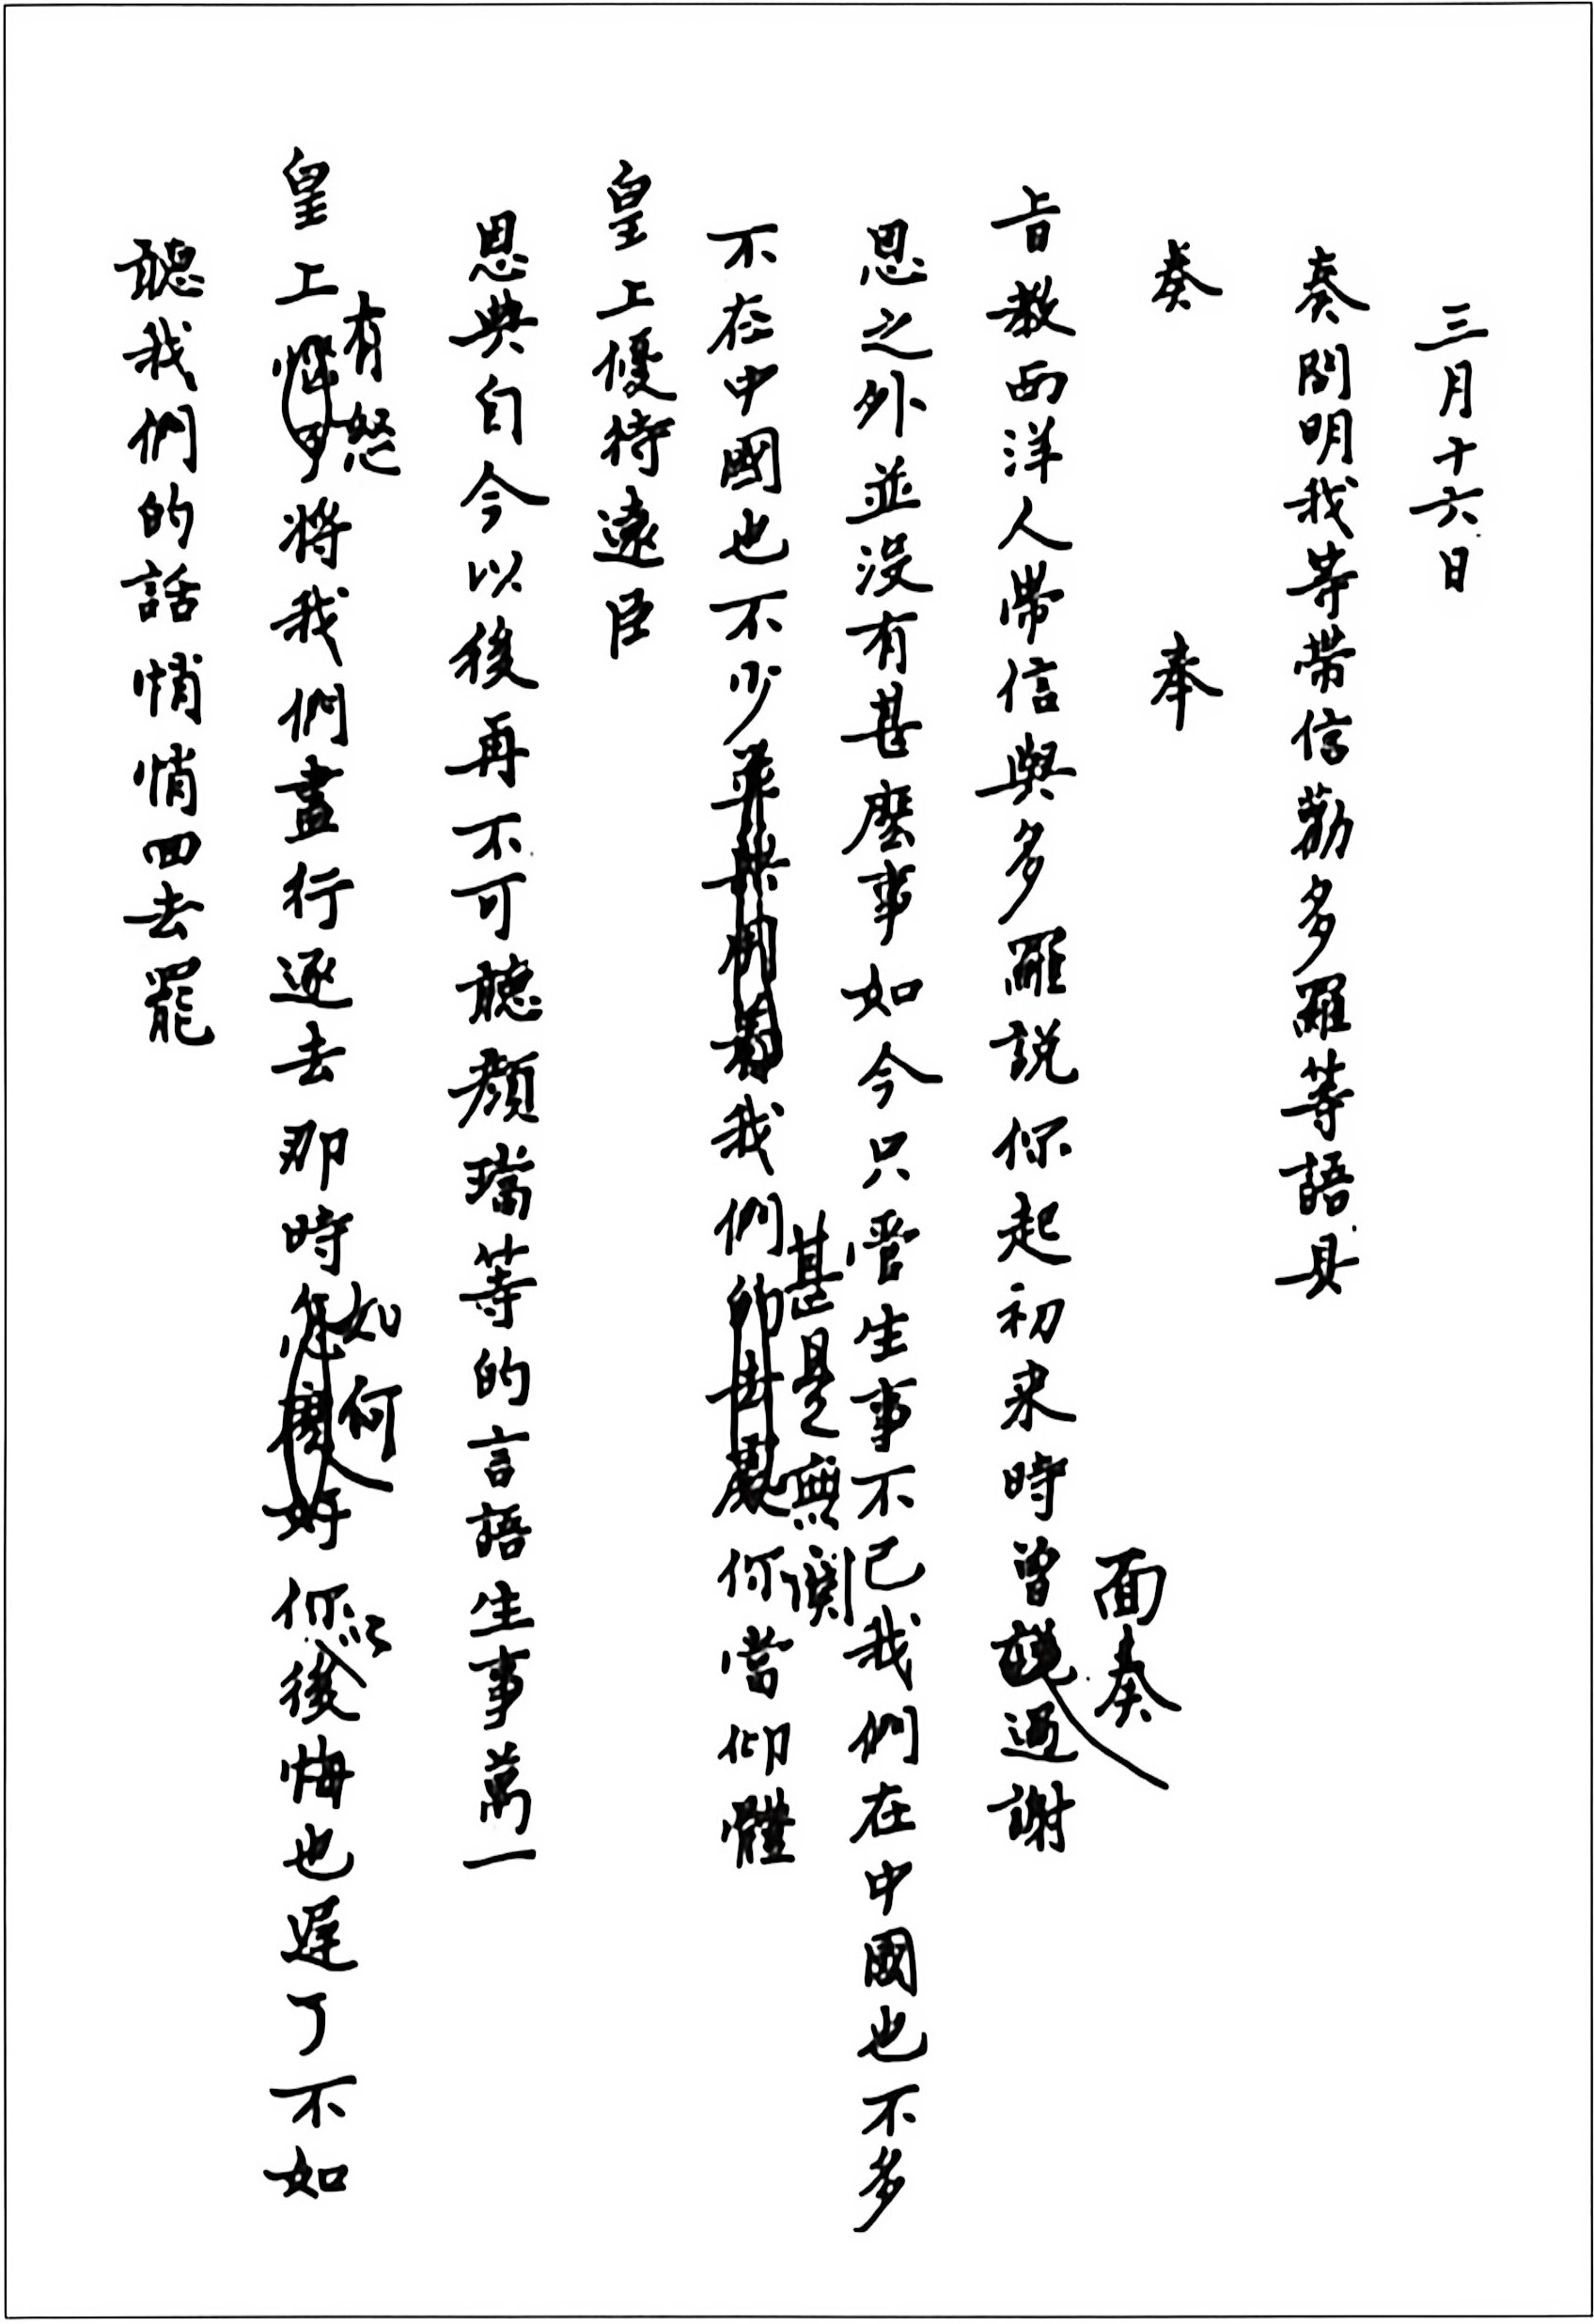
\includegraphics[width=\linewidth,height=.76\textheight,keepaspectratio]{assets/figures/kangxi-grimaldi-letter.png}
\caption*{图5.1\quad 康熙批改闵明我劝多罗信}
\BookFloatNotes{图片来源：陈垣编，《康熙与罗马使节关系文书》，文件3。}
\end{figure}%
不能辨别其真伪，康熙让礼部通过他们的渠道通知各地方。很快，%
地方上的传教士也发现他们领的印票在当地是有用的。在地方官眼%
里，这个票是内务府发的，相当于确认了这些传教士是康熙府中之%
人。无论从康熙规定领票的初衷还是后来的实际操作上看，康熙要%
求领票其实跟今天开车需要领驾照相类似，目的是为了规范，而不%
是为了限制。%
% 原书页码：200；标题
\subsection{小结}
\par
% 原书页码：200–201；段落（跨页续段）
民国时期，美国哈佛大学学者费正清在研究清代的外交中，提%
出了清朝的朝贡体系。其中最重要的一篇是20世纪40年代发表的%
总结清朝来华使团的论文，题目是《关于清朝的朝贡体系》。\NoteRef{5}{91}费正%
清总结了清代官方历史文献中的所有来华使团，他当时已经注意到，%
尽管清代的官方历史对各种大大小小的人华使团都有详细记录，但%
教皇派到康熙朝的使团竟然在大清所有的官修史书中都未见记载。%
俄罗斯派往康熙朝入京的使团有三个，但其中两个也都未见任何记%
录。而这几个未见记录的使团在西方文献中都很有名，费正清把它%
们单独列人一张表格中，但他没有能给出解释，为什么官修清史会%
出现选择性的记录和缺失。如果是因为别的原因，比如雍正不喜欢%
传教士，所以把教皇派到康熙朝的两个使团的记录删去了，那为什%
么所有的大清官修史书中，又都记录了教皇派到雍正朝的第三个使%
团？俄罗斯三次派到康熙朝的使团（1676、1693、1720）也是这样，%
其中第一次1676年的使团在清官修史书中有记录，而后面两次就没%
有任何记录。如果是有什么我们后人不知道的原因，又为什么只删%
除后面两次，而保留第一次？%
\par
% 原书页码：201；段落
我们知道了康熙接待多罗的各种细节以后，原因就一目了然了。%
没有记载并非后人的删除，而是因为康熙从一开始就把接待教皇使团%
当作他的家务事在操办，从头到尾都没有让朝廷部门经手。在康熙的%
安排下，整个过程都是他的内务府在一手操办，所以整个接待就不是%
外交活动了，而是他的家务事。因为是家务事，朝廷的史官自然就没%
有参与，也就没有留下记录。同样的原因，雍正在1725年接待教皇%
来使的时候，全程都交给了礼部在办理，属于朝廷接待，整个过程朝%
廷的史官都记录了。俄罗斯使团也是这个模式，第一次使团是礼部接%
待的，所以有记录，而后面两次都是康熙的内务府承办的。%
\par
% 原书页码：201；段落
康熙与耶稣会神父之间的关系决定了康熙接待教皇来使的各种安%
排。康熙在朝廷上是皇帝，而在他的家中，按照满人的传统，他是主%
子。他自然要照顾长期在他家庭圈子中的传教士。按康熙对传教士说%
的话，他同意接待多罗，是看在“豢养尔等多年”的分儿上。“豢养”%
二字在中文中是养家畜时使用的词语，特别是“豢”字，最早是用来%
表示喂猪（豕）的。满人主奴关系下，最早奴才和动物是一样的，主%
子负责奴才的吃喝，像养动物一样养奴才。在这个特殊的语境下，“豢%
养奴才”这样的表达才大量使用。%
\par
% 原书页码：201–202；段落（跨页续段）
最后康熙决定用内务府把多罗使团当成私人关系接待，接待中%
吃吃喝喝，都是很典型的满人主子宴请待客之道。多罗后来慢慢明%
白了康熙和耶稣会神父之间的关系后，很无奈，因为无论他和康熙%
说什么，耶稣会神父都要按照他们的想法给康熙分析一遍。多罗在%
一封信中说道：“耶稣会神父在宝座的背后，为了他们的自私想法，%
误导着皇帝。”\NoteRef{5}{92}%
\par
% 原书页码：202；段落
康熙对耶稣会神父的信任，从中国历史上来看都是很不寻常的。%
比如他决定派遣使节到欧洲，选派的人员都是听他周围耶稣会神父推%
荐的。其中的薄贤士没有在康熙身边当过差，康熙只是看过他写的对%
中国礼仪问题的论说，就决定选派他代表自已出使。薄贤士自己都有%
些意外，在谢恩中特别感谢康熙的信任。\NoteRef{5}{93}3康熙对待耶稣会神父的一%
切都是基于他和这些神父长久以来的私人关系。这和礼仪问题及天主%
教教义都没有多大关系。他容纳天主教也好，接见多罗也好，都是看%
在他周围神父的面子上的。所以只要他和这些神父的关系不变，他对%
天主教的态度也不会有大的变化。对于多罗来讲，他的出使在最后阶%
段失败了，他人华的所有目的都没有达到。但是对于耶稣会神父和康%
熙来说，与罗马的交流才刚刚开始。康熙派出的两个去罗马的使节带%
着希望出发了。%
